\documentclass[12pt]{report} %fuente a 12pt

% MÁRGENES: 2,5 cm sup. e inf.; 3 cm izdo. y dcho.
\usepackage[
a4paper,
vmargin=2.5cm,
hmargin=3cm
]{geometry}

% INTERLINEADO: Estrecho (6 ptos./interlineado 1,15) o Moderado (6 ptos./interlineado 1,5)
\renewcommand{\baselinestretch}{1.15}
\parskip=6pt

% DEFINICIÓN DE COLORES para portada y listados de código
\usepackage[table]{xcolor}
\definecolor{azulUC3M}{RGB}{0,0,102}
\definecolor{gray97}{gray}{.97}
\definecolor{gray75}{gray}{.75}
\definecolor{gray45}{gray}{.45}

% Soporte para GENERAR PDF/A
\usepackage[a-1b]{pdfx}

% ENLACES
\usepackage{hyperref}
\hypersetup{colorlinks=true,
	linkcolor=black, % enlaces a partes del documento (p.e. índice) en color negro
	urlcolor=blue} % enlaces a recursos fuera del documento en azul

\usepackage{pdfpages}
\setlength{\parindent}{0em}

% EXPRESIONES MATEMATICAS
\usepackage{amsmath,amssymb,amsfonts,amsthm}

\usepackage{txfonts} 
\usepackage[T1]{fontenc}
\usepackage[utf8]{inputenc}

\usepackage{tikz}
\usepackage{pgfplots}

\usepackage[spanish, es-tabla]{babel} 
\usepackage[babel, spanish=spanish]{csquotes}
\AtBeginEnvironment{quote}{\small}

% diseño de PIE DE PÁGINA
\usepackage{fancyhdr}
\pagestyle{fancy}
\fancyhf{}
\renewcommand{\headrulewidth}{0pt}
\rfoot{\thepage}
\fancypagestyle{plain}{\pagestyle{fancy}}

% DISEÑO DE LOS TÍTULOS de las partes del trabajo (capítulos y epígrafes o subcapítulos)
\usepackage{titlesec}
\usepackage{titletoc}
\titleformat{\chapter}[block]
{\large\bfseries\filcenter}
{\thechapter.}
{5pt}
{\MakeUppercase}
{}
\titlespacing{\chapter}{0pt}{0pt}{*3}
\titlecontents{chapter}
[0pt]                                               
{}
{\contentsmargin{0pt}\thecontentslabel.\enspace\uppercase}
{\contentsmargin{0pt}\uppercase}                        
{\titlerule*[.7pc]{.}\contentspage}                 

\titleformat{\section}
{\bfseries}
{\thesection.}
{5pt}
{}
\titlecontents{section}
[5pt]                                               
{}
{\contentsmargin{0pt}\thecontentslabel.\enspace}
{\contentsmargin{0pt}}
{\titlerule*[.7pc]{.}\contentspage}

\titleformat{\subsection}
{\normalsize\bfseries}
{\thesubsection.}
{5pt}
{}
\titlecontents{subsection}
[10pt]                                               
{}
{\contentsmargin{0pt}                          
	\thecontentslabel.\enspace}
{\contentsmargin{0pt}}                        
{\titlerule*[.7pc]{.}\contentspage}  


% DISEÑO DE TABLAS.
\usepackage{multirow} % permite combinar celdas 
\usepackage{caption} % para personalizar el título de tablas y figuras
\usepackage{floatrow} % utilizamos este paquete y sus macros \ttabbox y \ffigbox para alinear los nombres de tablas y figuras de acuerdo con el estilo definido. Para su uso ver archivo de ejemplo 
\usepackage{array} % con este paquete podemos definir en la siguiente línea un nuevo tipo de columna para tablas: ancho personalizado y contenido centrado
\newcolumntype{P}[1]{>{\centering\arraybackslash}p{#1}}
\DeclareCaptionFormat{upper}{#1#2\uppercase{#3}\par}

% Diseño de tabla para ingeniería
\captionsetup[table]{
	format=upper,
	name=TABLA,
	justification=centering,
	labelsep=period,
	width=.75\linewidth,
	labelfont=small,
	font=small,
}

% DISEÑO DE FIGURAS.
\usepackage{graphicx}
\graphicspath{{img/}} %ruta a la carpeta de imágenes

% Diseño de figuras para ingeniería
\captionsetup[figure]{
	format=hang,
	name=Fig.,
	singlelinecheck=off,
	labelsep=period,
	labelfont=small,
	font=small		
}

% NOTAS A PIE DE PÁGINA
\usepackage{chngcntr} %para numeración continua de las notas al pie
\counterwithout{footnote}{chapter}

% LISTADOS DE CÓDIGO
% soporte y estilo para listados de código. Más información en https://es.wikibooks.org/wiki/Manual_de_LaTeX/Listados_de_código/Listados_con_listings
\usepackage{listings}

% definimos un estilo de listings
\lstdefinestyle{estilo}{ frame=Ltb,
	framerule=0pt,
	aboveskip=0.5cm,
	framextopmargin=3pt,
	framexbottommargin=3pt,
	framexleftmargin=0.4cm,
	framesep=0pt,
	rulesep=.4pt,
	backgroundcolor=\color{gray97},
	rulesepcolor=\color{black},
	%
	basicstyle=\ttfamily\footnotesize,
	keywordstyle=\bfseries,
	stringstyle=\ttfamily,
	showstringspaces = false,
	commentstyle=\color{gray45},     
	%
	numbers=left,
	numbersep=15pt,
	numberstyle=\tiny,
	numberfirstline = false,
	breaklines=true,
	xleftmargin=\parindent
}

\captionsetup[lstlisting]{font=small, labelsep=period}
% fijamos el estilo a utilizar 
\lstset{style=estilo}
\renewcommand{\lstlistingname}{\uppercase{Código}}

\pgfplotsset{compat=1.17} 
%-------------
%	DOCUMENTO
%-------------

\begin{document}
\pagenumbering{roman} % Se utilizan cifras romanas en la numeración de las páginas previas al cuerpo del trabajo
	
%----------
%	PORTADA
%----------	
\begin{titlepage}
	\begin{sffamily}
	\color{azulUC3M}
	\begin{center}
		\begin{figure}[H] %incluimos el logotipo de la Universidad
			\makebox[\textwidth][c]{
\includegraphics[width=16cm]{Portada_Logo.png}}
		\end{figure}
		\vspace{2.5cm}
		\begin{Large}
			Grado en Ingeniería Informática\\			
			2020-2021\\
			\vspace{2cm}		
			\textsl{Apuntes}\\
			\bigskip
		\end{Large}
		 	{\Huge Aprendizaje Automático}\\
		 	\vspace*{0.5cm}
	 		\rule{10.5cm}{0.1mm}\\
			\vspace*{0.9cm}
			{\LARGE Jorge Rodríguez Fraile\footnote{\href{mailto:100405951@alumnos.uc3m.es}{Universidad: 100405951@alumnos.uc3m.es}  |  \href{mailto:jrf1616@gmail.com}{Personal: jrf1616@gmail.com}}}\\ 
			\vspace*{1cm}
	\end{center}
	\vfill
	\color{black}
		
\includegraphics[width=4.2cm]{img/creativecommons.png}\\
		Esta obra se encuentra sujeta a la licencia Creative Commons\\ \textbf{Reconocimiento - No Comercial - Sin Obra Derivada}
	\end{sffamily}
\end{titlepage}

%----------
%	ÍNDICES
%----------	

%--
% Índice general
%-
\tableofcontents
\thispagestyle{fancy}

%--
% Índice de figuras. Si no se incluyen, comenta las líneas siguientes
%-
\listoffigures
\thispagestyle{fancy}

%--
% Índice de tablas. Si no se incluyen, comenta las líneas siguientes
%-
\listoftables
\thispagestyle{fancy}

%----------
%	TRABAJO
%----------	
\clearpage
\pagenumbering{arabic} % numeración con números arábigos para el resto de la publicación	


%----------
%	COMENZAR A ESCRIBIR AQUI
%----------	


\section{Información}

\begin{quote}
Teorías: Raquel Fuentetaja rfuentet@inf.uc3m.es 2.1B19

Prácticas: Rubén Majadas rmajadas@pa.uc3m.es 2.2A12
\end{quote}

\section{Presentación}

Vamos a trabajar sobre una modificación del Pac-man.

Los fantasmas no van a por Pac-man, si no que si los toca se los come.

Las practicas consisten en 4 Tutoriales 0.5 cada uno y 2 Practicas 1.5
cada una.

El objetivo de la asignatura es conseguir que gane solo el Pac-man sin
ayuda nuestra.

El objetivo de las practicas no es pegar los resultados o con captura,
si no documentar bien, incluyendo tablas y graficas.

Los casos que no funcionan son importantes, no solo poner pruebas con
éxito. Así se documentan los cambios realizados.

\section{Recursos}

\chapter{TEMA 1. Introducción}

\textbf{Definición}:

Campo de estudio que da al computador la habilidad de aprender.

Un programa se dice que aprende de una experiencia con respecto a una
tarea y alguna medida del rendimiento, si el rendimiento con la tarea al
ser medido mejora con la experiencia.

\textbf{Objetivo}: Aprender conocimiento nuevo y mejorar el
comportamiento de un sistema.

Se encuentra en las fronteras de la programación.

\textbf{Programación tradicional}: Lo normal, es que el usuario
construya el programa que resuelve el problema.

\begin{figure}[H]
	\ffigbox[\FBwidth]
	{\caption{Programación tradicional}}
	{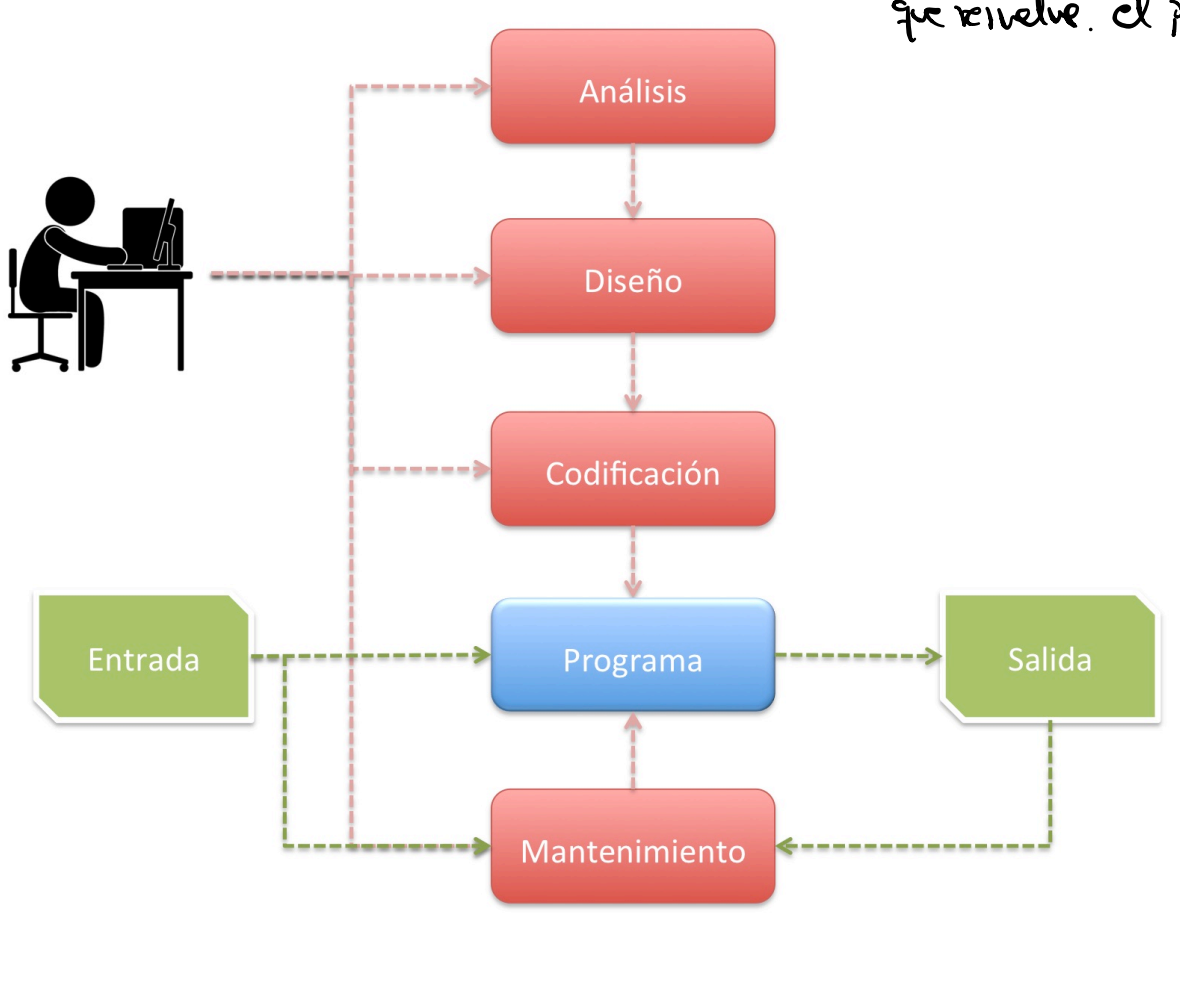
\includegraphics[scale=.15]{Untitled.png}}
\end{figure}

\textbf{Programación automática}: Se crea un programa capaz de generar
el programa que es capaz de resolver nuestro problema.

\begin{figure}[H]
	\ffigbox[\FBwidth]
	{\caption{Programación automática}}
	{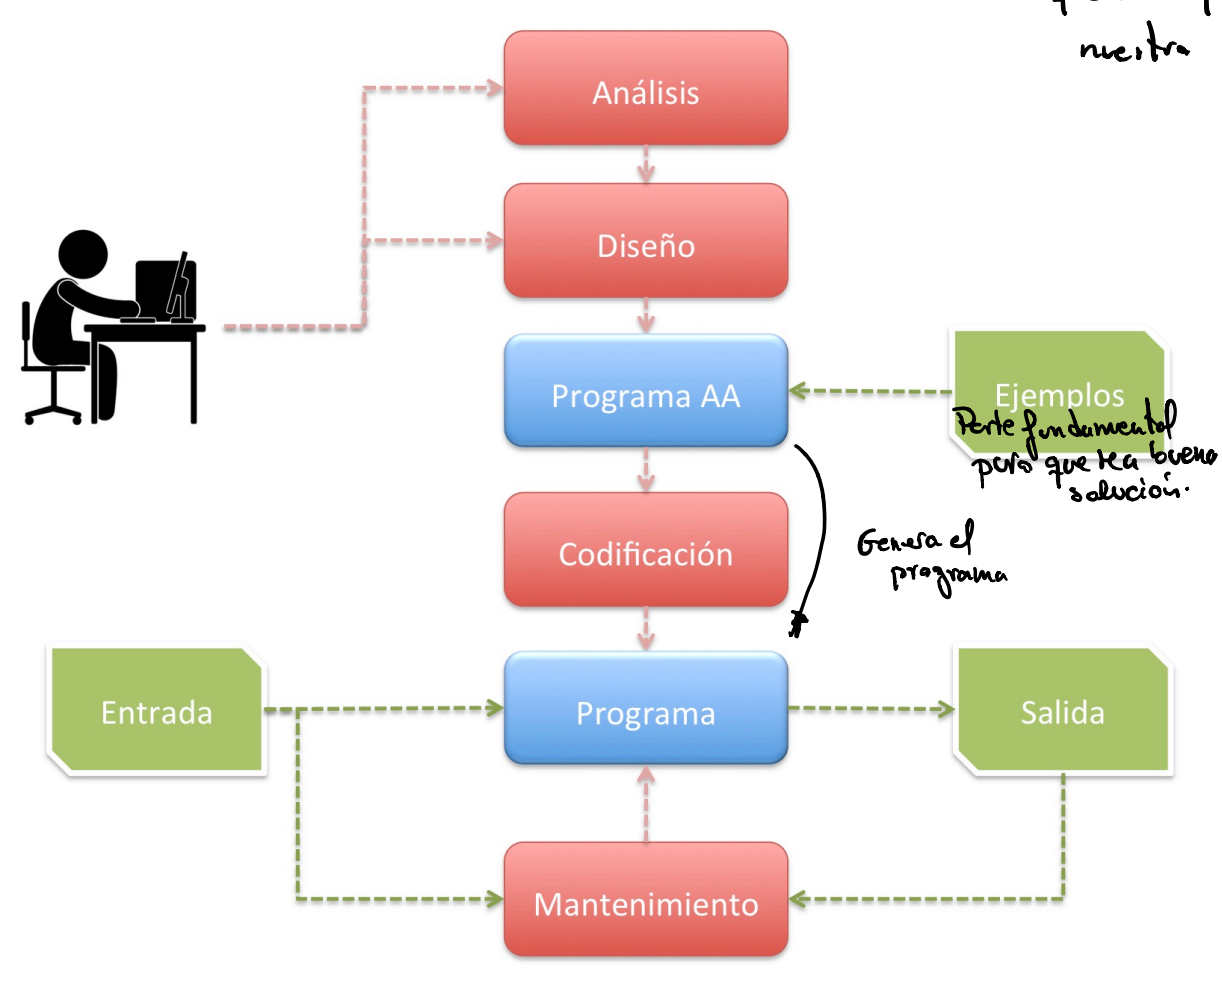
\includegraphics[scale=.15]{Untitled 1.png}}
\end{figure}

\newpage

\textbf{Es útil cuando:}

\begin{itemize}
\item
  No existe experiencia humana.
\item
  Los humano no saben explicar su experiencia.
\item
  Los modelos deben ser personalizados
\item
  Los modelos se basan en enormes cantidades de datos.
\end{itemize}

\textbf{Actualmente}: Existen muchos algoritmos de aprendizaje
automático efectivo y eficientes, recursos computacionales y datos
disponibles.

\textbf{Definición de tarea de Aprendizaje Automático}: Mejorar en una
\textbf{tarea} T, respecto a una \textbf{medida de rendimiento} P,
basándose en la \textbf{experiencia} E (los ejemplos).

Tarea, Medida y Experiencia.

\begin{figure}[H]
	\ffigbox[\FBwidth]
	{\caption{Tipos de tareas de Aprendizaje Automático}}
	{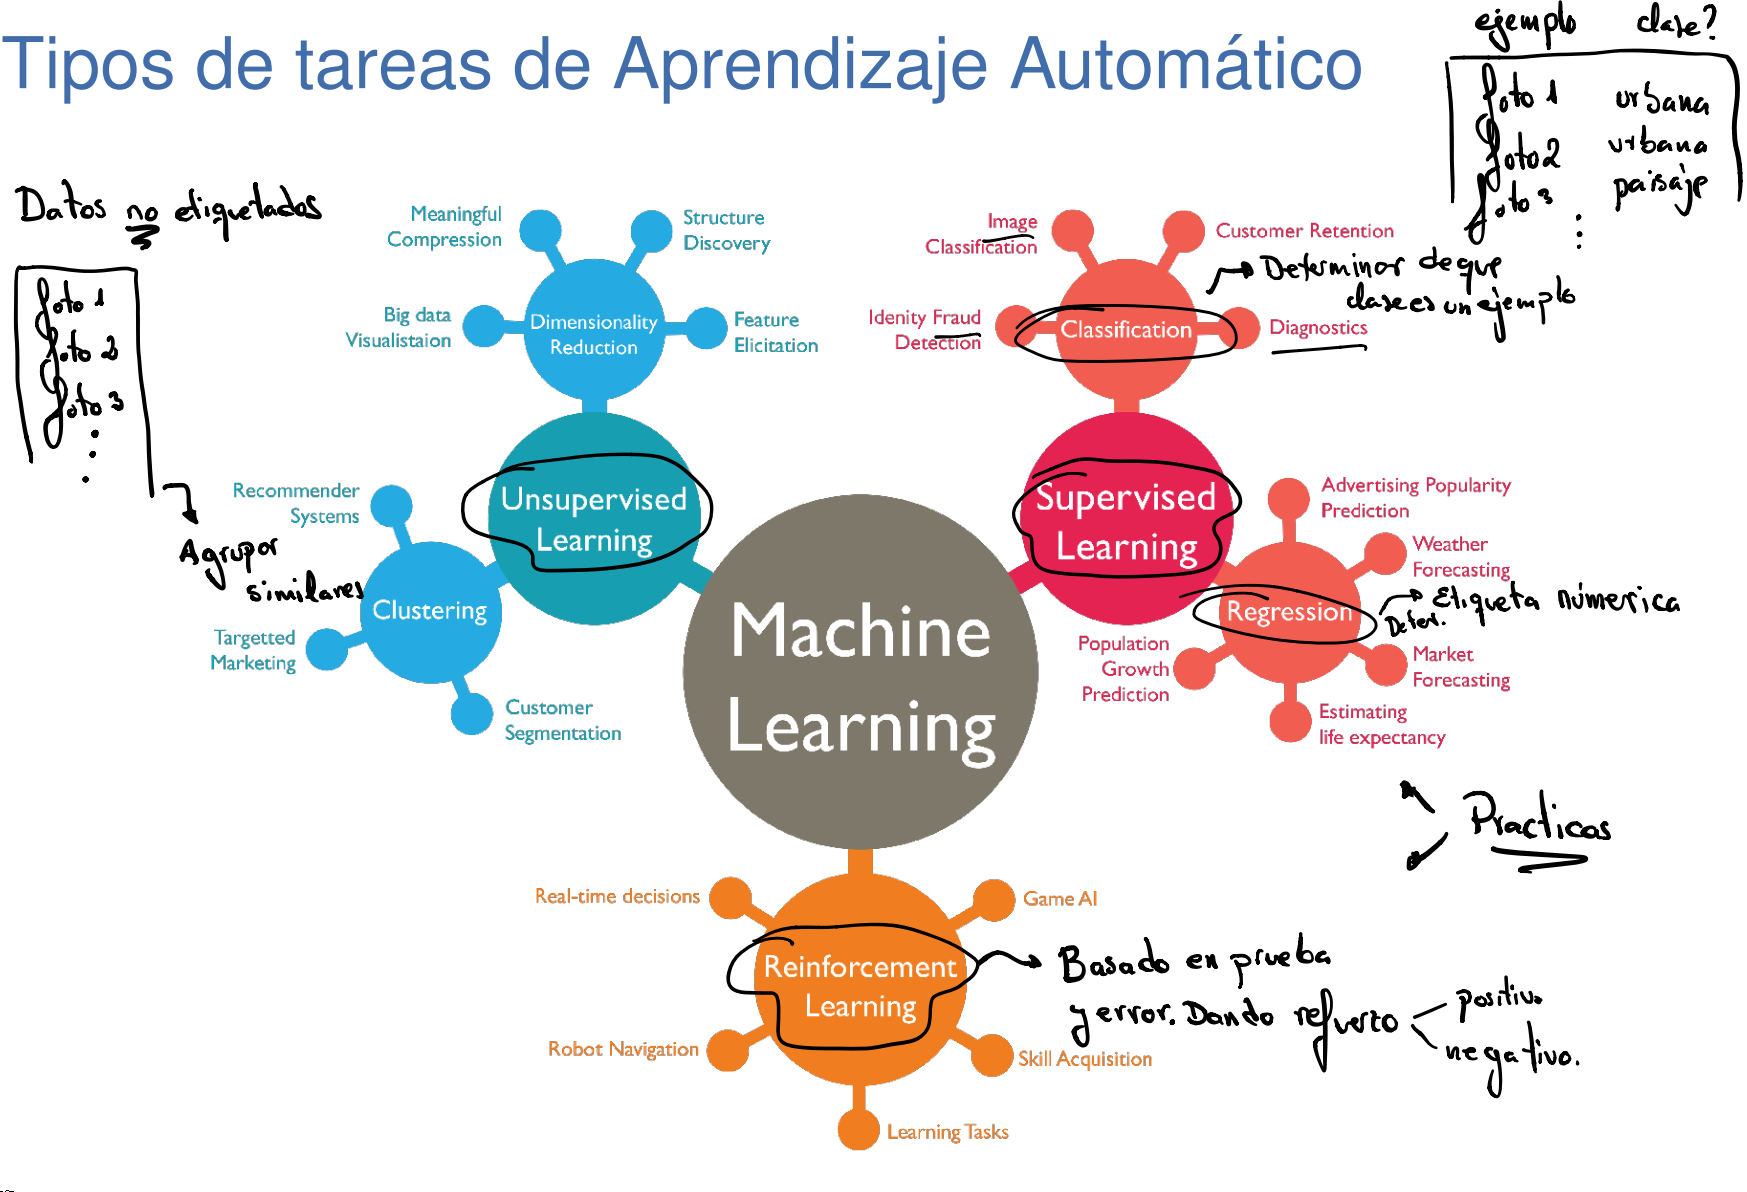
\includegraphics[scale=.2]{Untitled 2.png}}
\end{figure}
\textbf{Tipos de tareas de Aprendizaje Automático:}



\begin{itemize}

\item
  \textbf{Aprendizaje supervisado}: Consiste en etiquetar los datos.

  \begin{itemize}
  
  \item
    \textbf{Clasificación}: Determinar de qué clase es un ejemplo.
    
  \item
    \textbf{Predicción -- Regresión}: Determinar una etiqueta numérica.

  \end{itemize}
\item
  \textbf{Aprendizaje no supervisado}: Agrupa elementos similares, no
  etiqueta.

  \begin{itemize}
  
  \item
    \textbf{Agrupación}.
  \end{itemize}
\item
  \textbf{Aprendizaje por refuerzo}: Basado en prueba y error. Dando
  refuerzo positivo/negativo.
\end{itemize}

\textbf{Algunas aplicaciones}: Sanidad, Domótica, Banca, Marketing,
Personalización, Seguridad, Videojuego, etc.

\textbf{Problemas no técnicos:}

\begin{itemize}
\item
  Las maquinas no son responsables de los diagnósticos, predicciones, o
  clasificaciones que hacen.
\item
  Los humanos no se fían de los resultados .
\item
  La salida no es entendible por el humano. No explica sus decisiones,
  se está avanzando para lograr saber cómo piensa.
\item
  Leyes de protección de datos.
\item
  Miedo de los humanos a la pérdida de control.
\item
  Cuestiones éticas.
\end{itemize}

\chapter{TEMA 2. Árboles y Reglas de
Decisión}

\section{Aprendizaje inductivo (De lo más específico a lo más
general)}

Encontrar una \textbf{función h} (la hipótesis o modelo) que aproxime la
\textbf{función f} (desconocida) definida por un conjunto de ejemplos.

Los ejemplos normalmente se representan como pares, \textbf{(x, f(x))}.

\textbf{Según como sea la salida de f}: Es \textbf{clasificación} si es
categórica y es de \textbf{regresión} si es numérica.

Se basa en inducción, se parte de un ejemplo específico para obtener
modelos generales.

\textbf{Asume que:}

\begin{itemize}
\item
  La \textbf{hipótesis del aprendizaje es inductiva.}
\item
  Si un modelo o hipótesis \textbf{categoriza bien en función a un
  conjunto de ejemplos grande también lo hará bien para futuros
  ejemplos.}
\item
  \textbf{Siempre hay un sesgo inductivo}, que influye en la decisión,
  nos lleva más a uno que a otro.
\item
  El lenguaje de representación nos limita si no lo puede expresar bien.
  Por ejemplo, limitarnos a una función lineal, pero es cuadrática.
\item
  Encontrar una hipótesis adecuada puede ser difícil, f es desconocida y
  puede ser complicado determinar si h es buena.
\end{itemize}

El \textbf{espacio de hipótesis} es el conjunto de hipótesis que se
consideran para aproximar f, \textbf{influye mucho para encontrar una
buena aproximación}, pueden ser: funciones lineales, polinómicas, lógica
de predicados, arboles de decisión, etc.

Los ejemplos tienen atributos/características que los identifican y nos
permitirán clasificarlos por clases. Cada ejemplo es una instancia, da
valor a los atributos y su clase.

Todos los ejemplos clasificados forman el conjunto de entrenamiento.

\section{Definiciones}

\textbf{Atributos}: Característica que define a un elemento de un
conjunto.

\textbf{Instancia}: Colección de valores de atributos.

\textbf{Clase}: Cada uno de los subconjuntos disjuntos.

\textbf{Ejemplo (positivo)}: Instancia que pertenece al subconjunto
definido por la clase.

\textbf{Ejemplo negativo}: No pertenece al subconjunto definido por la
clase.

\textbf{Generalización de un conjunto de ejemplos de una
clase(hipótesis)}: Descripción que representa al subconjunto de
instancias de la clase y no de otras.

\section{Arboles y reglas de
decisión}

Usaremos \textbf{modelos simbólicos como arboles de decisión}, que usa
símbolos para representar lo que los hace más fáciles para ver
explicaciones de las decisiones, lo entendemos. Sin embargo, en otros
tipos de modelos como los numéricos (redes neuronales), usa números para
representar y no es posible que dé explicaciones que entendamos.

\section{Aprendizaje de árboles de
decisión}

Nosotros estudiaremos \textbf{ID3 (Dicotomizador Iterativo, Quinlan
1986)}, a partir de ejemplos de partida genera arboles de decisión.
Normalmente NO son arboles binarios.

Usa búsqueda avara, para encontrar el árbol más sencillo que separa
mejor los ejemplos. Utiliza una heurística basada en entropía. Trata de
escoger para empezar la clasificación el atributo que mejor separa las
distintas clases.

\section{Algoritmo}

\begin{enumerate}
\def\labelenumi{\arabic{enumi}.}
\item
  \textbf{Seleccionar el atributo} \(A_i\) que maximice la ganancia
  \(G(A_i)\).
\item
  \textbf{Crear un nodo} para ese atributo con \textbf{tantos sucesores
  como valores} tenga.
\item
  \textbf{Dividir los ejemplos} en los sucesores según el valor del
  atributo.
\item
  Por cada sucesor,

  sí solo hay \textbf{ejemplo de una clase}, entonces se
  \textbf{etiqueta con esa clase},

  si no, \textbf{ejecutar el ID3} con la tabla formada por los ejemplos
  de ese nodo, pero sin el atributo que todos tiene en común.
\end{enumerate}

  Ejemplo:
\begin{figure}[H]
	\ffigbox[\FBwidth]
	{\caption{Diagramas ID3 I}}
	{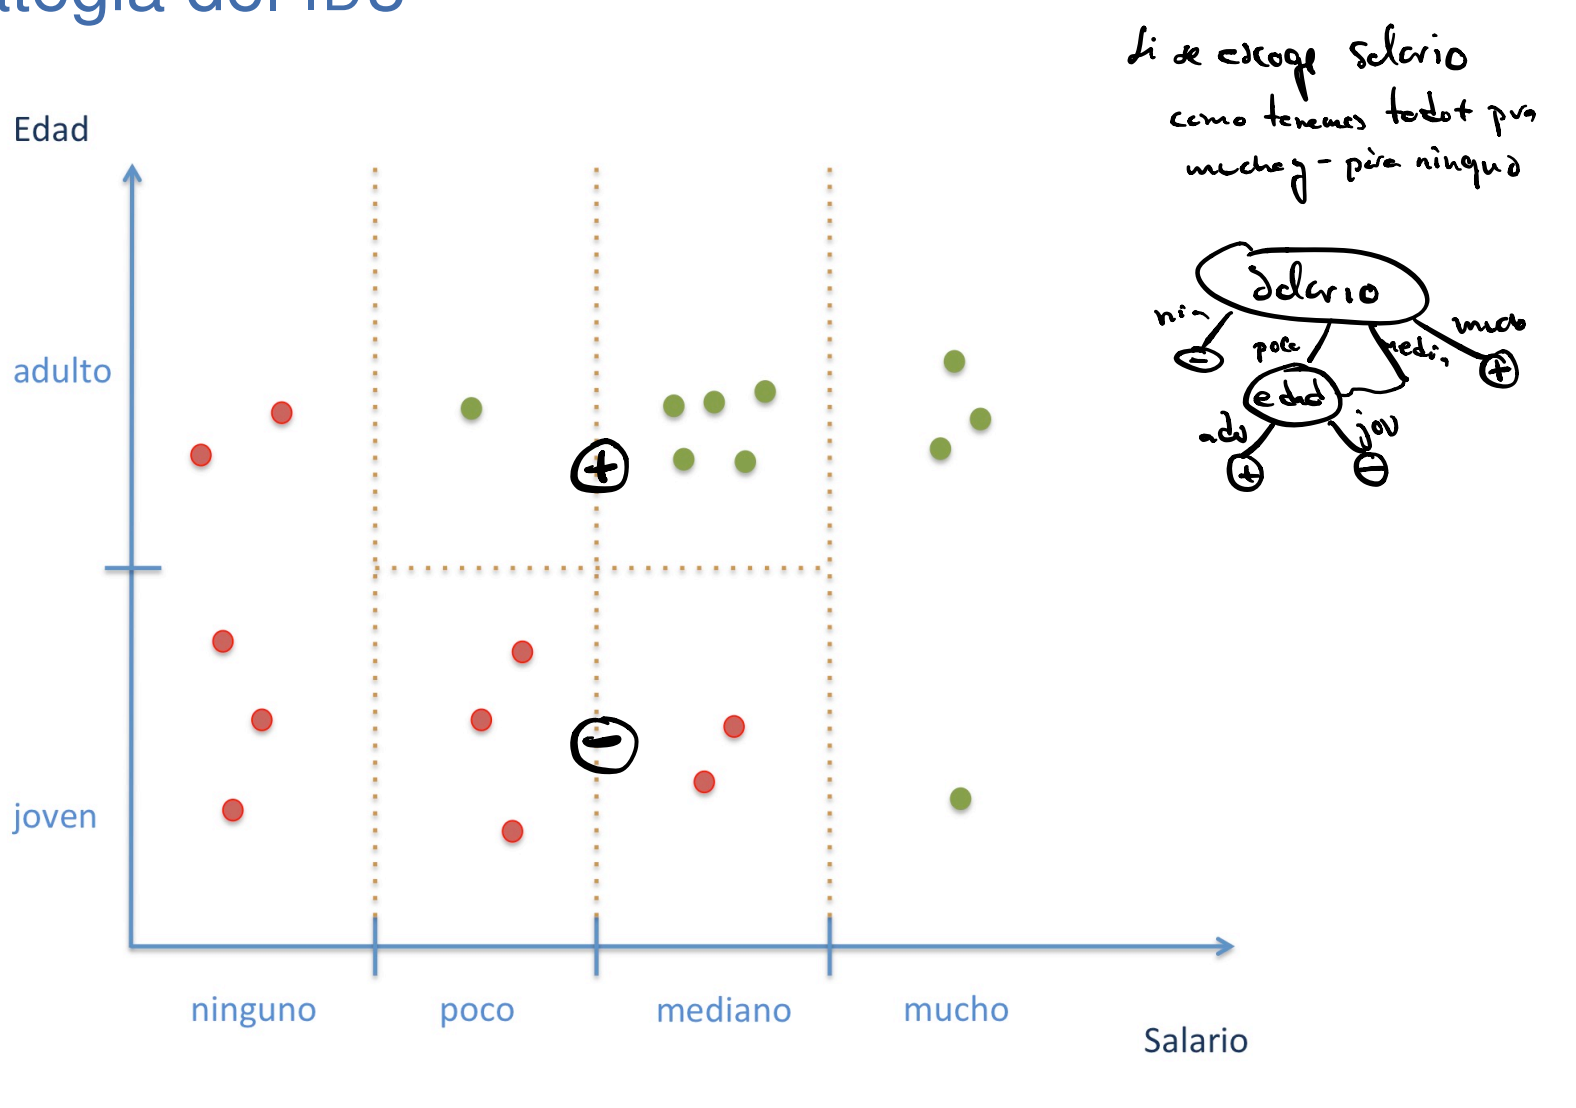
\includegraphics[scale=.2]{Untitled 3.png}}
\end{figure}
\begin{figure}[H]
	\ffigbox[\FBwidth]
	{\caption{Diagramas ID3 II}}
	{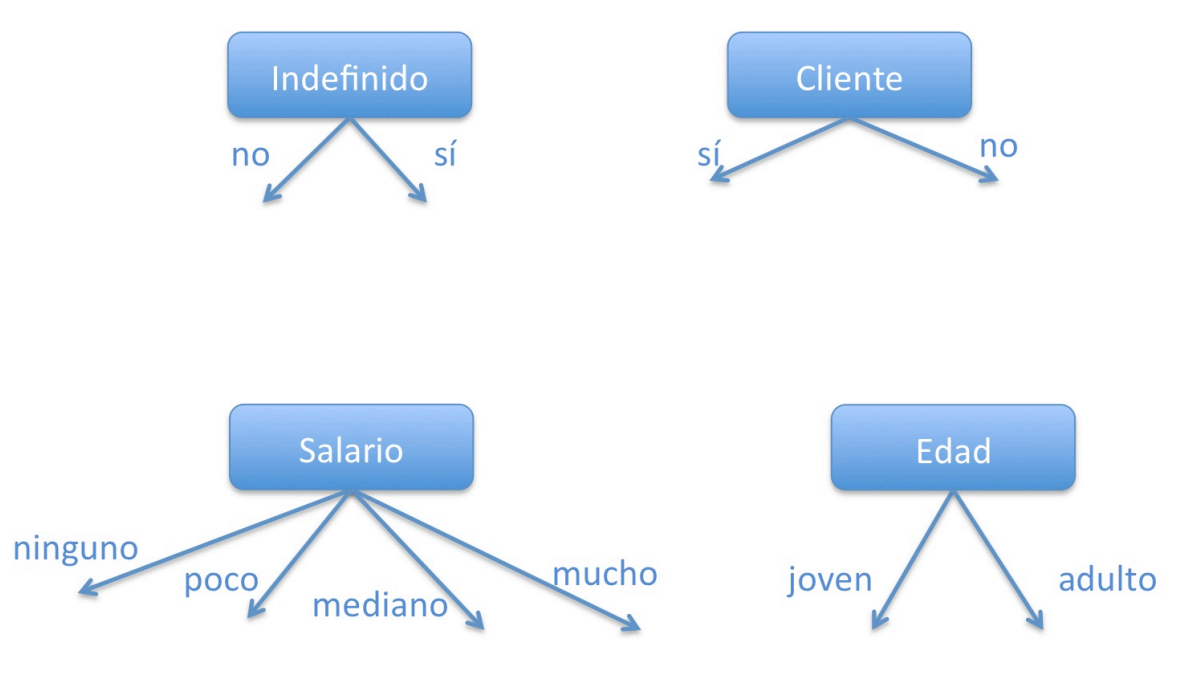
\includegraphics[scale=.2]{Untitled 4.png}}

\end{figure}
\begin{figure}[H]
	\ffigbox[\FBwidth]
	{\caption{Diagramas ID3 III}}
	{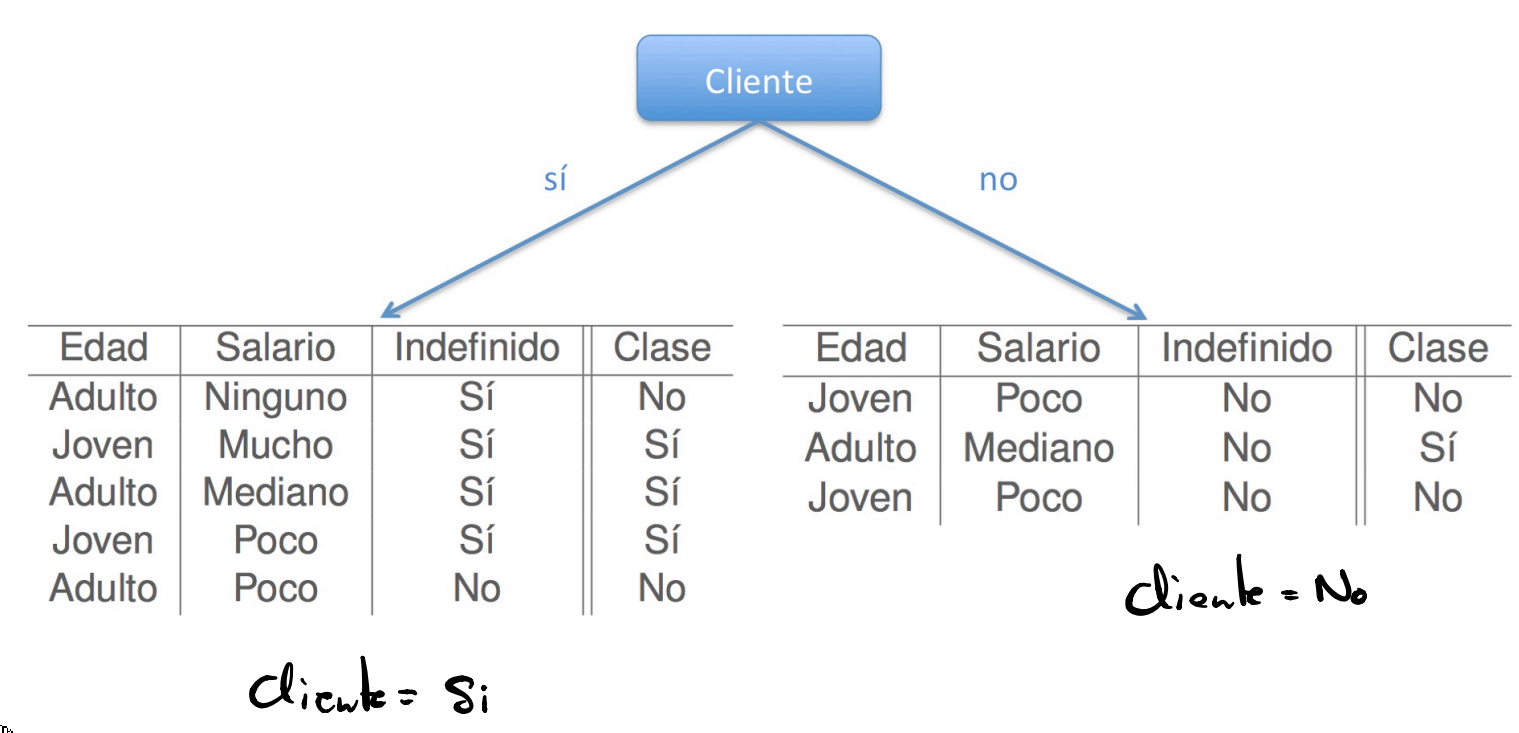
\includegraphics[scale=.2]{Untitled 5.png}}
\end{figure}
\begin{figure}[H]
	\ffigbox[\FBwidth]
	{\caption{Diagramas ID3 IV}}
	{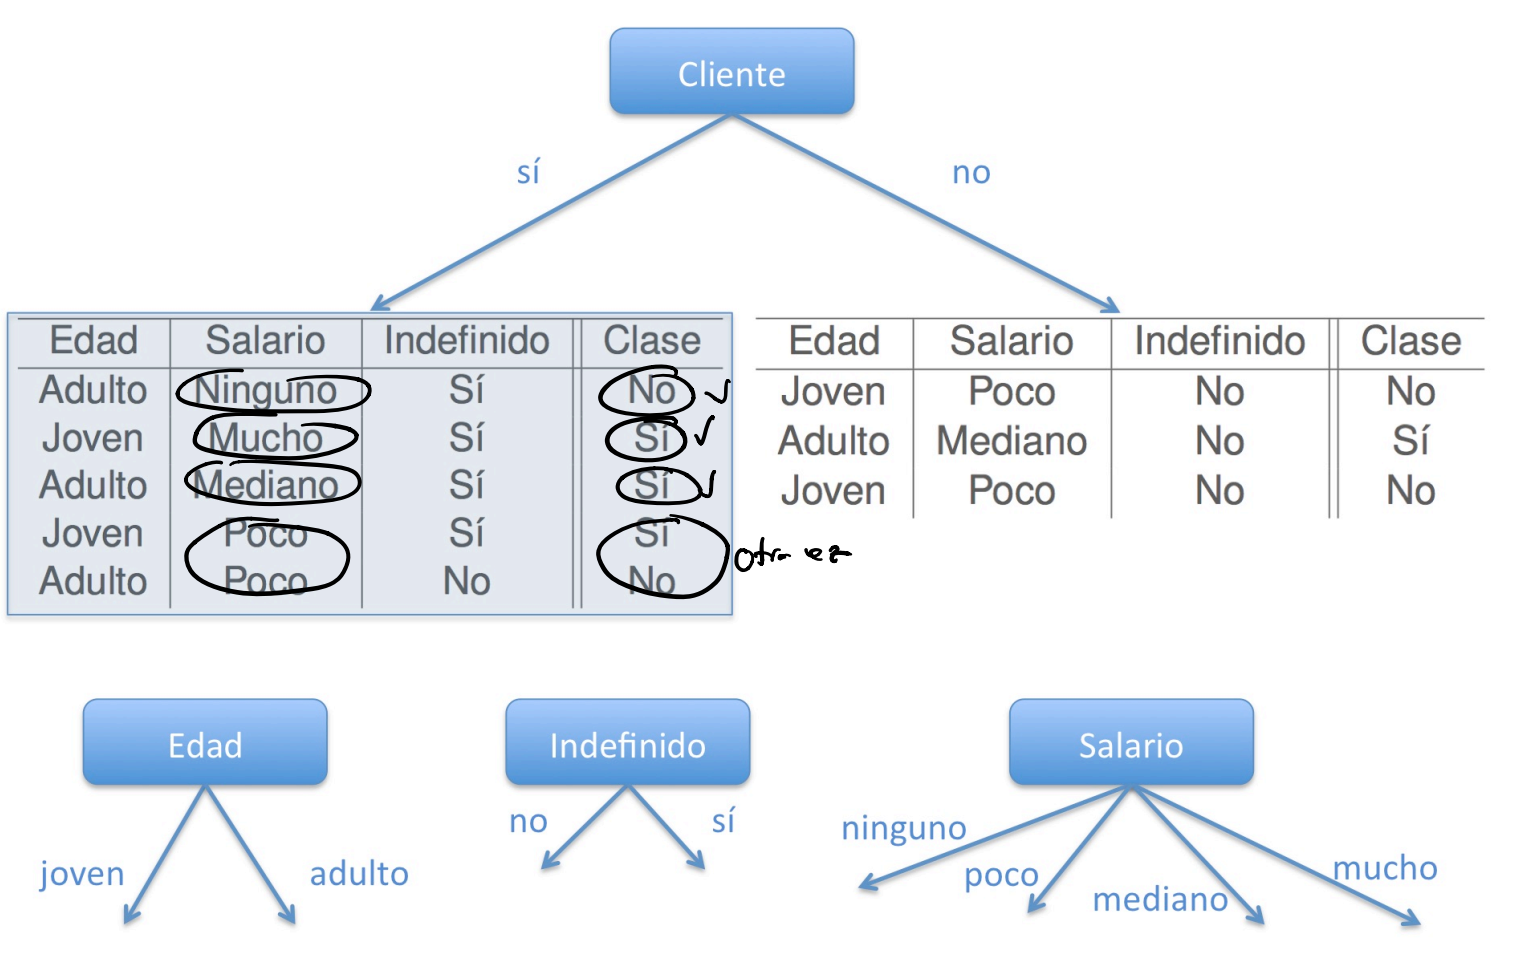
\includegraphics[scale=.2]{Untitled 6.png}}
\end{figure}
\begin{figure}[H]
	\ffigbox[\FBwidth]
	{\caption{Diagramas ID3 V}}
	{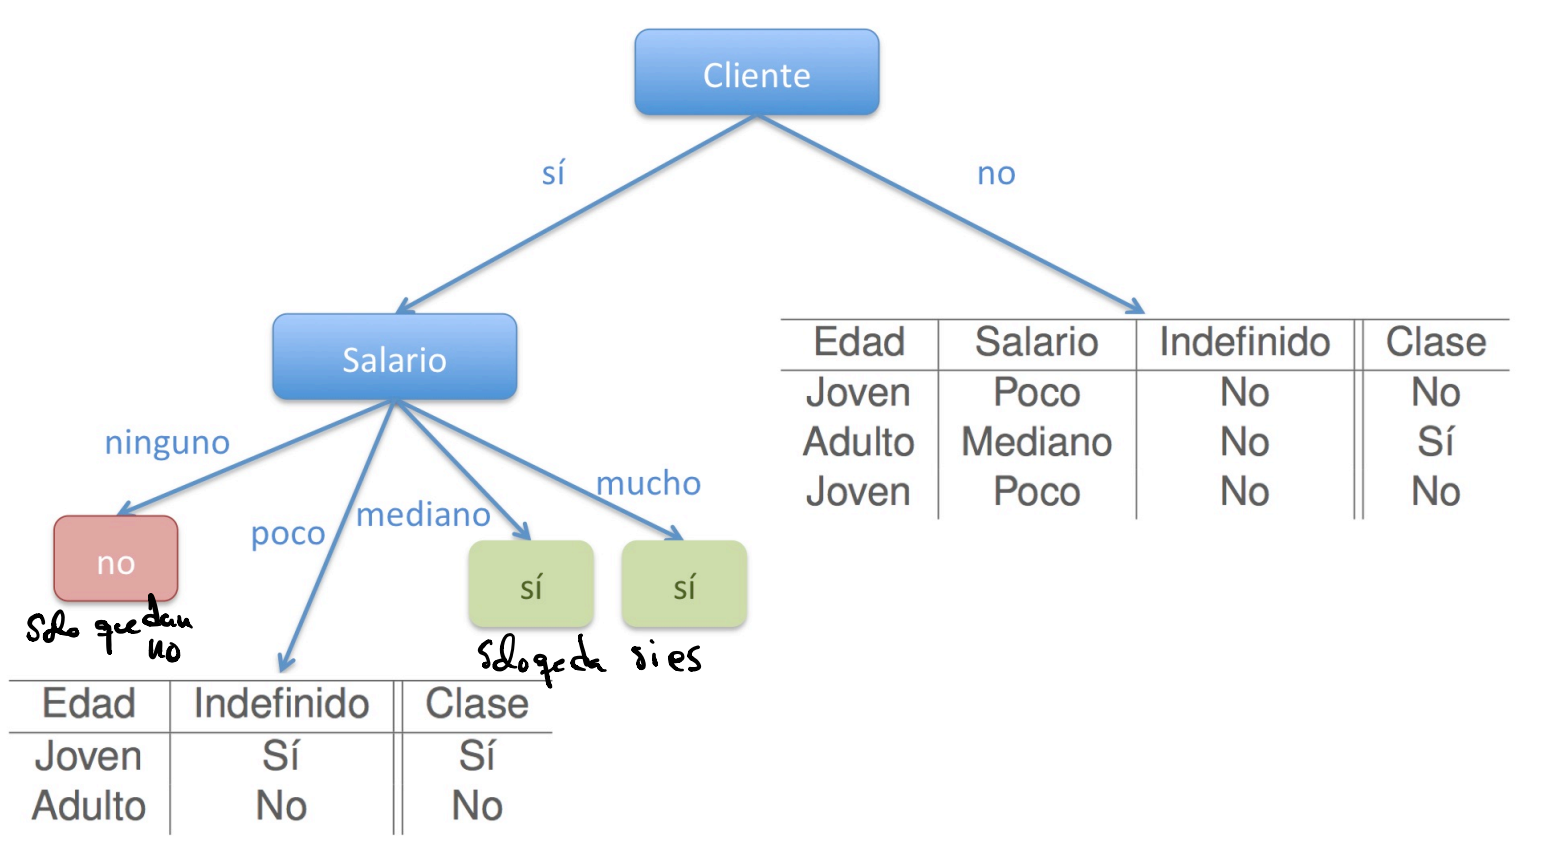
\includegraphics[scale=.2]{Untitled 7.png}}
\end{figure}
\begin{figure}[H]
	\ffigbox[\FBwidth]
	{\caption{Diagramas ID3 VI}}
	{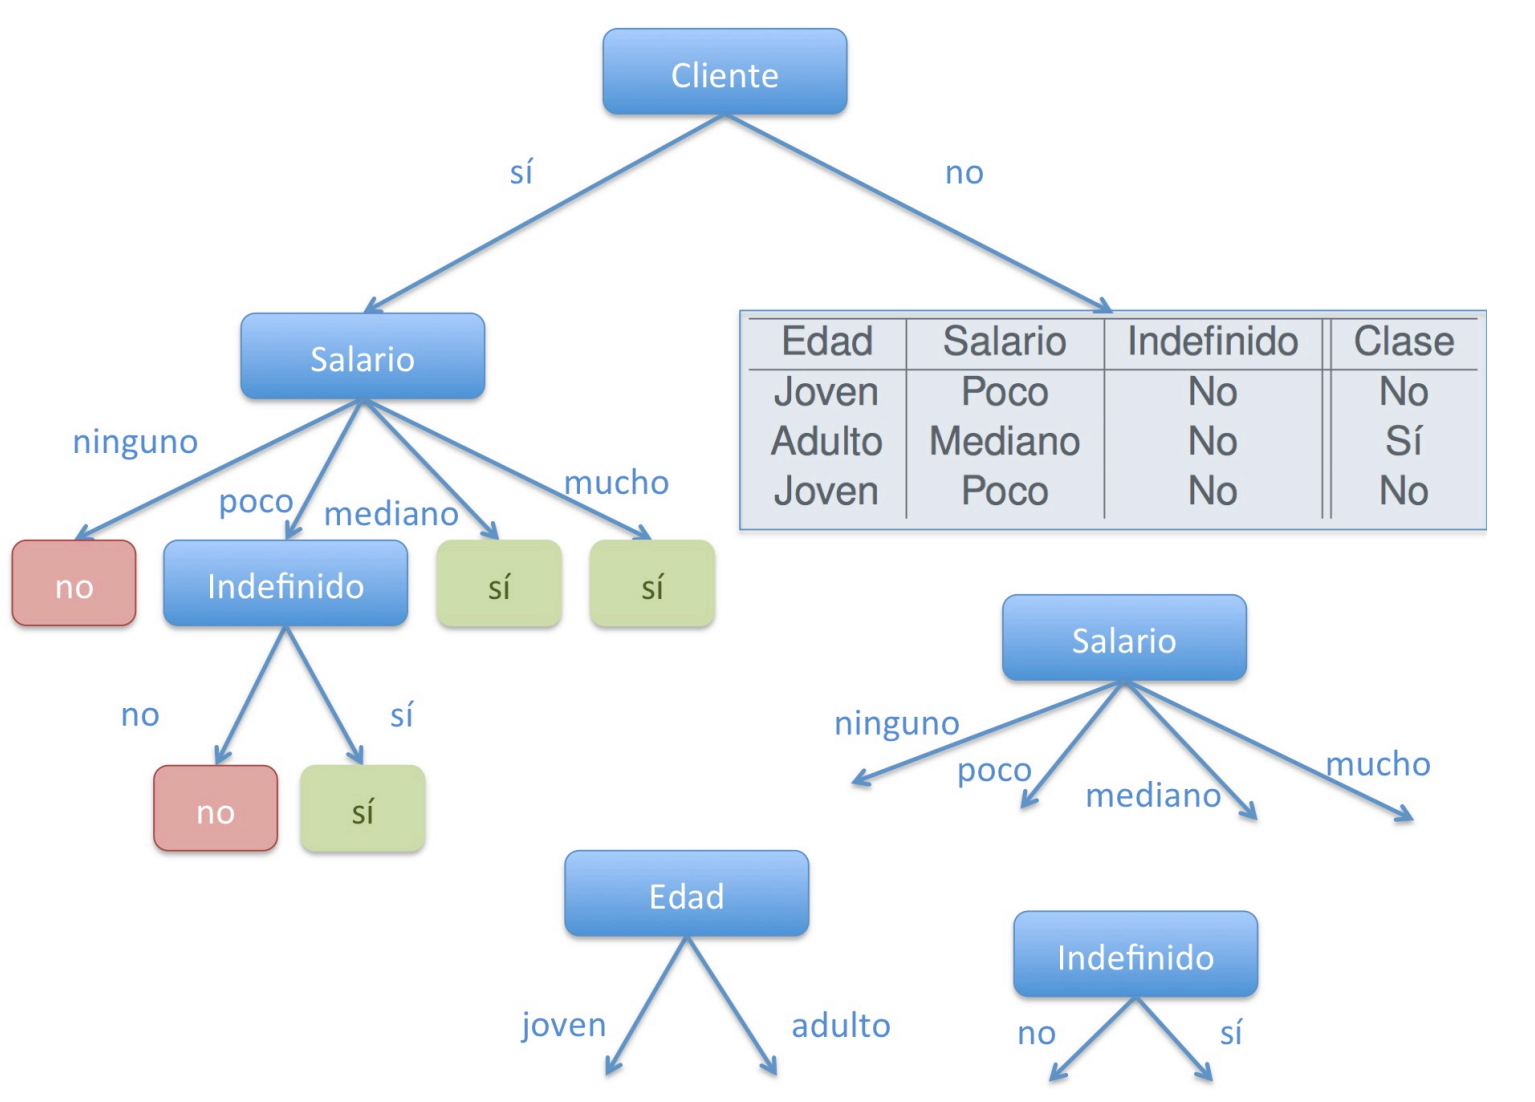
\includegraphics[scale=.2]{Untitled 8.png}}
\end{figure}
\begin{figure}[H]
	\ffigbox[\FBwidth]
	{\caption{Diagramas ID3 VII}}
	{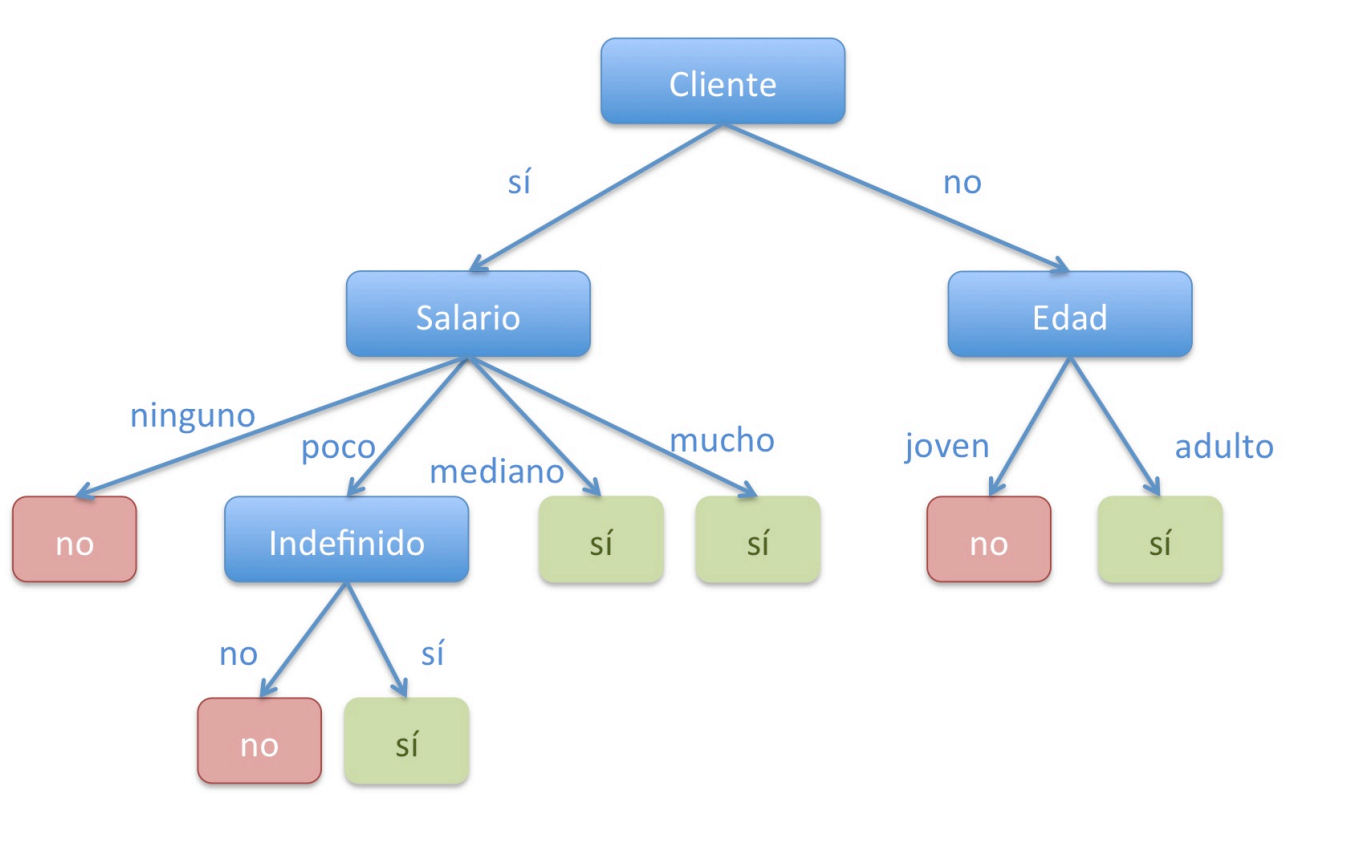
\includegraphics[scale=.2]{Untitled 9.png}}
\end{figure}


\section{Heurística de ID3 (Heurística de la ganancia de
información)}

Seleccionar el \textbf{atributo que mejor separe los ejemplos de acuerdo
con las clases}, que deje subconjuntos más puros (orientados más a un
valor)

Para calcular la ganancia se utiliza el concepto de Entropía, como
medida de la pureza o impureza de un conjunto ejemplos.
\newpage
\section{Entropía}

\textbf{Entropía en clasificación binaria}: El conjunto de ejemplos S
pertenece a una de las dos clases:
\textbf{\(Entropia(S) \equiv -p_\oplus \log _2 p_\oplus -p_\ominus \log _2 p_\ominus\)}

\begin{itemize}
\item
  \(p_\oplus\): \textbf{Proporción} de ejemplos \textbf{positivos} sobre
  el total.
\item
  \(p_\ominus\): \textbf{Proporción} de ejemplos \textbf{negativos}
  sobre el total.
\end{itemize}

\(p_\oplus+p_\ominus=1\)

\(p_\oplus+p_\ominus=0.5\) Entropía máxima

\textbf{Entropía en múltiples clases}:
\(Entropia(S) \equiv \sum_{c\in C} -p_c \log _2 p_c\)

Cuanto más se diferencian las proporciones, cuanto más notablemente hay de una que de otra, más tiende a 0.

\textbf{Nuestro objetivo es minimizar la entropía.}

\textbf{La ganancia de información:} mide la efectividad de un atributo
para clasificar, es la \textbf{reducción esperada de la entropía} cuando
se divide el conjunto de datos original S según el atributo dado A.

\begin{itemize}
\item
  \(G(S,A)=Entropia(S) - Entropia\_ Atr(S,A)\)
\item
  \(Entropia\_ Atr(S,A)= \sum_{c \in valores(A)} \frac {|S_{A=v}|}{|S|} Entropia(S_{A=v})\)
\item
  \(Entropia(S_{A=v})= -\sum_{c \in C} \frac {|S_{A=v,C=c}|}{|_{A=v}|} \log_2 \frac {|S_{A=v,C=c}|}{|_{A=v}|}\)
\end{itemize}

\textbf{Se elige el atributo que maximiza la ganancia de información},
ya que menos resta es el que menos entropía tiene, o elegir el que menor
\textbf{entropía tenga}.

\(A= \arg\max_{A \in \mathcal{A}} G(S,A) = \arg\min_{A \in \mathcal{A}} Entropia \_ Atr(A,S)\)


\begin{figure}[H]
	Ejemplo
	\ffigbox[\FBwidth]
	{\caption{Ejemplo cálculo de entropía}}
	{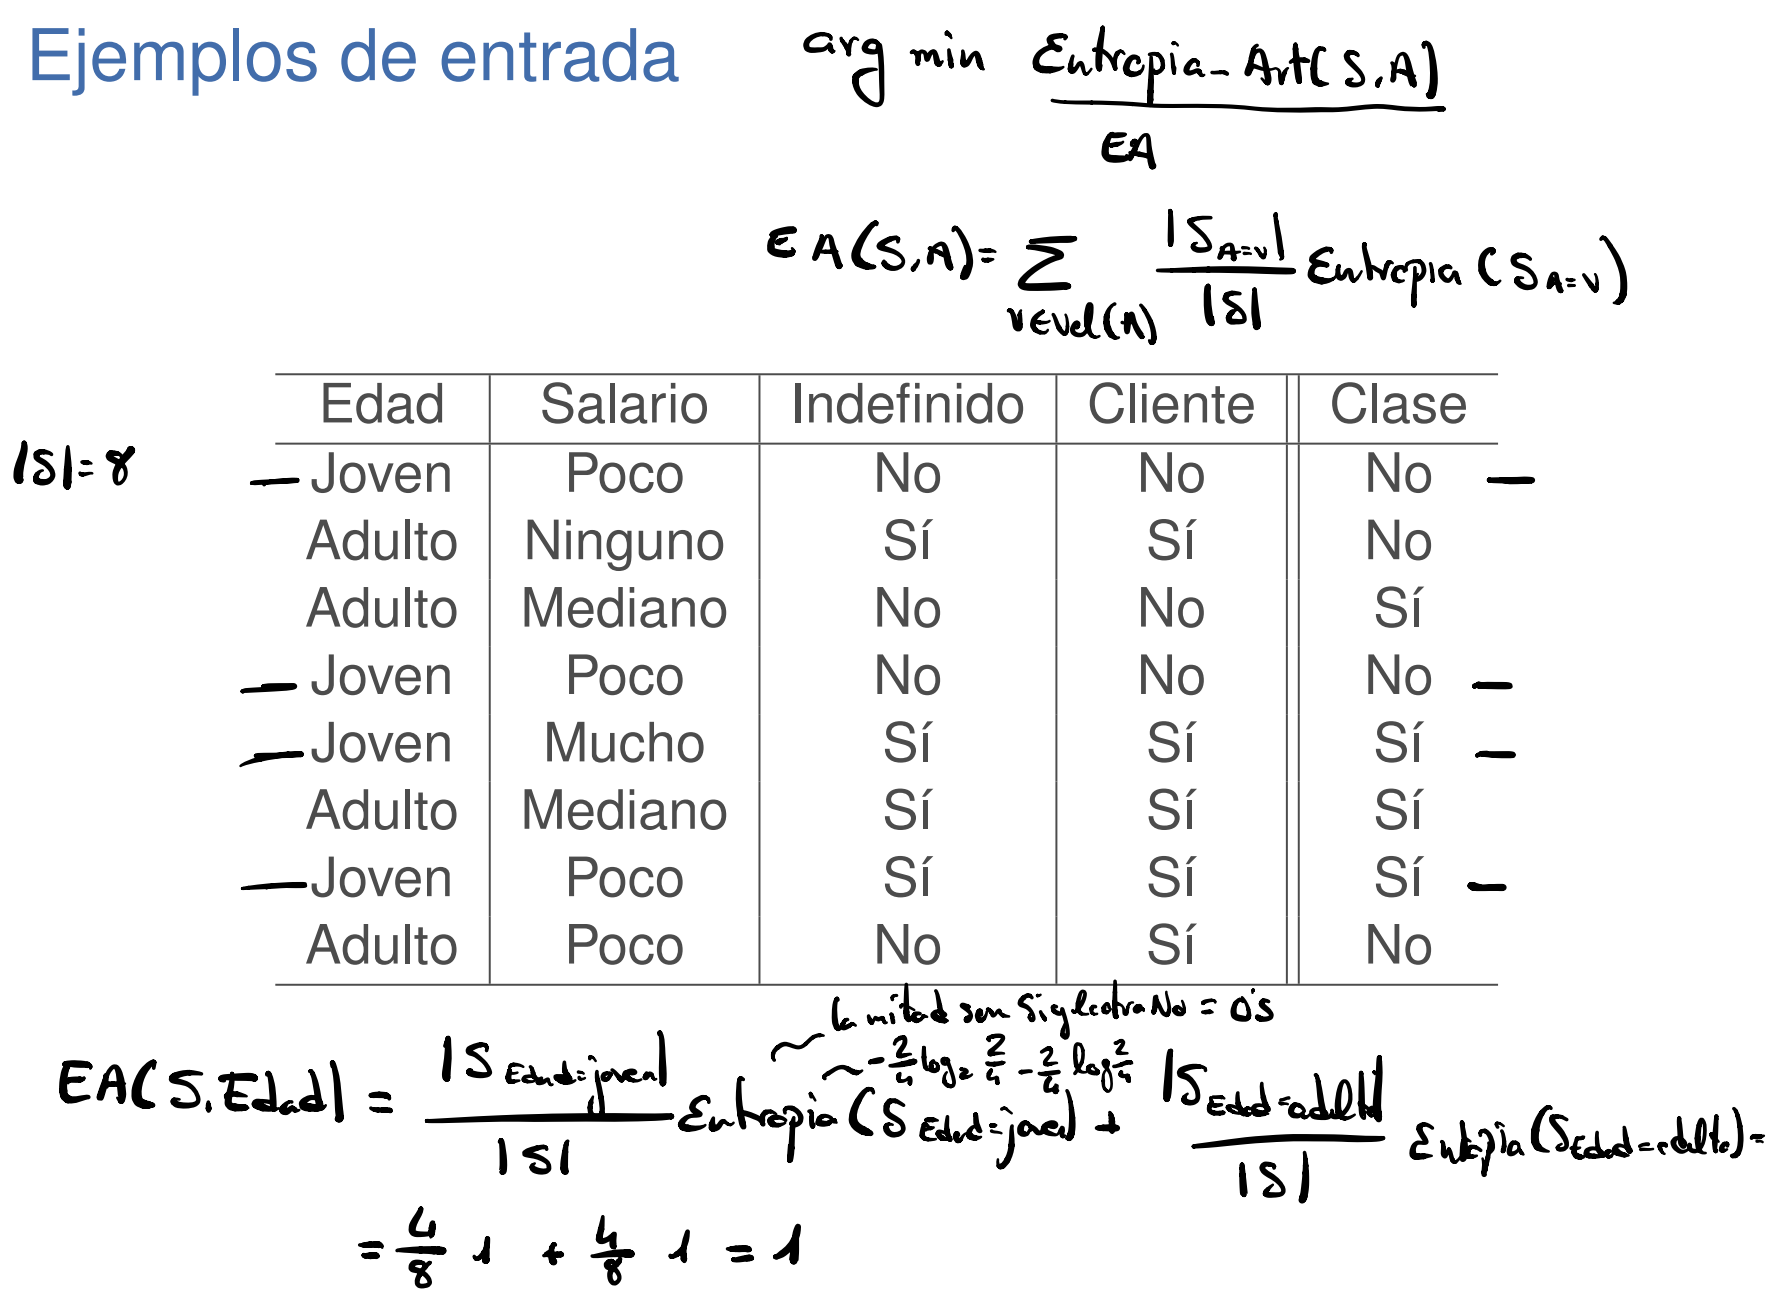
\includegraphics[scale=.15]{Untitled 10.png}}
\end{figure}


\section{Aprendizaje de reglas de
decisión}

\textbf{Traducción a reglas:}

\begin{itemize}
\item
  Cualquier árbol de decisión se puede convertir a reglas.
\item
  \textbf{Reglas}: Estructura del tipo \textbf{Si(valor de los
  atributos)-Entonces(clase a la que pertenece)}
\item
  \textbf{Algoritmo}: Por cada rama del árbol, las preguntas y sus
  valores estarán en la parte de la izquierda de las reglas y la
  etiqueta del nodo hoja correspondiente será la parte derecha.
\end{itemize}

\textbf{Sesgo inductivo en ID3}

\begin{itemize}
\item
  Preferir arboles con atributos con más información cerca de la raíz, y
  arboles cortos.
\item
  \textbf{La navaja de Ockham/Occam:} Preferir siempre la hipótesis más
  sencilla que describa los datos.
\item
  Favorece atributos con muchos valores.
\end{itemize}

\section{Ampliación del ID3}

En los datos puede haber errores, ruido. Si se ajusta mucho a los datos
se produce \textbf{sobreajuste}.

\textbf{No se pueden tratar:}

\begin{itemize}

\item
  \textbf{Valores continuos de atributos}, números reales, lo que no son
  discretos.
\item
  \textbf{Valores discretos con muchos valores.}
\end{itemize}

Hay valores de atributos más caros de obtener.

\begin{itemize}
\item
  Hay métodos que los ejemplos vienen incrementalmente, se puede ampliar
  el modelo, no hace falta volver a empezar: ID4, ID5 y Hoeffding tree.
\item
  Clases continuas: M5
\item
  Representación relacional, la más común es con lógica de predicados:
  ILP.
\end{itemize}

Normalmente recibimos los datos como \textbf{atributo-valor}, esta forma
es \textbf{proposicional}.

\section{Ruido}

Cualquier cosa que pueda oscurecer la relación entre los atributos y la
clase.

\begin{itemize}

\item
  Que los atributos no estén bien descritos o seleccionados.
\item
  Que no sean relevantes los atributos.
\end{itemize}

\textbf{Ruido en atributos:} Valores erróneos, sin valor (missing
values) o outliers (que se salen de sus valores)

\textbf{Ruido en la clase:} Ejemplos con una clase incorrecta, ejemplos
exactamente iguales, pero clase distinta (contradictorio)

\section{Evaluación para Validación de un
modelo}

No se pueden usar para evaluar ejemplos conocidos, tienen que ser
nuevos, para ello se tienen \textbf{dos conjuntos de ejemplos, uno para
entrenar y otros de prueba}. Tras crear el modelo se pasan los ejemplos
de prueba y se calcula el número de errores, se evalúan los resultados.

\(Accuracy= \frac {numeroEjemplosClasificadosCorrectamente}{numeroTotalEjemplos}\)
Proporción de aciertos sobre conjunto de prueba.

Un problema de hacer la división de conjuntos es que no se usan todos
para entrenar, y esto es problemático si no se tienen muchos.

\textbf{Validación cruzada k-veces:} Método para definir el conjunto de
entrenamiento y de pruebas, que permite usar todos los datos para
entrenar el modelo. Sirve para \textbf{estimar el error del modelo
final, no para generar el modelo final}, en el que se usan todos los
ejemplos.

Estimación del error del modelo final, en el que se usan todos los
ejemplos para entrenarlo.

\begin{enumerate}
\def\labelenumi{\arabic{enumi}.}

\item
  Divide el \textbf{conjunto de ejemplos en k partes} iguales.
\item
  Para cada conjunto, se \textbf{entrena con los k-1 conjuntos
  restantes}, y se pasa por el modelo generado el conjunto seleccionado
  calculando el error de ese modelo sobre el conjunto. \(e_i\)
\item
  Se estima la \textbf{tasa de error total haciendo la media} aritmética
  de los errores. \(r= \sum_{i=1}^k \frac {e_i}{k}\)
\end{enumerate}

Si k=5, se hacen 5 modelos (clasificadores) para evaluar y otro que es
el final que usa todos. k=n entonces n+1 modelos.

El valor de \textbf{k típico es 10}, pero la mejor sería que fuese
`Leave one out'(aunque es muy lento y costoso), coger todas menos 1
instancia para entrenar y usar esa para hacer test.

\section{Medidas adicionales del
rendimiento}

Tener una precisión alta, no quiere decir que sea bueno, la clase puede
estar desbalanceada, que haya más de una clase que otra, aunque se
admite cierta diferencia.

\textbf{Basadas en la Matriz de confusión:}

\begin{figure}[H]
	\ffigbox[\FBwidth]
	{\caption{Matriz de confusión con fórmulas}}
	{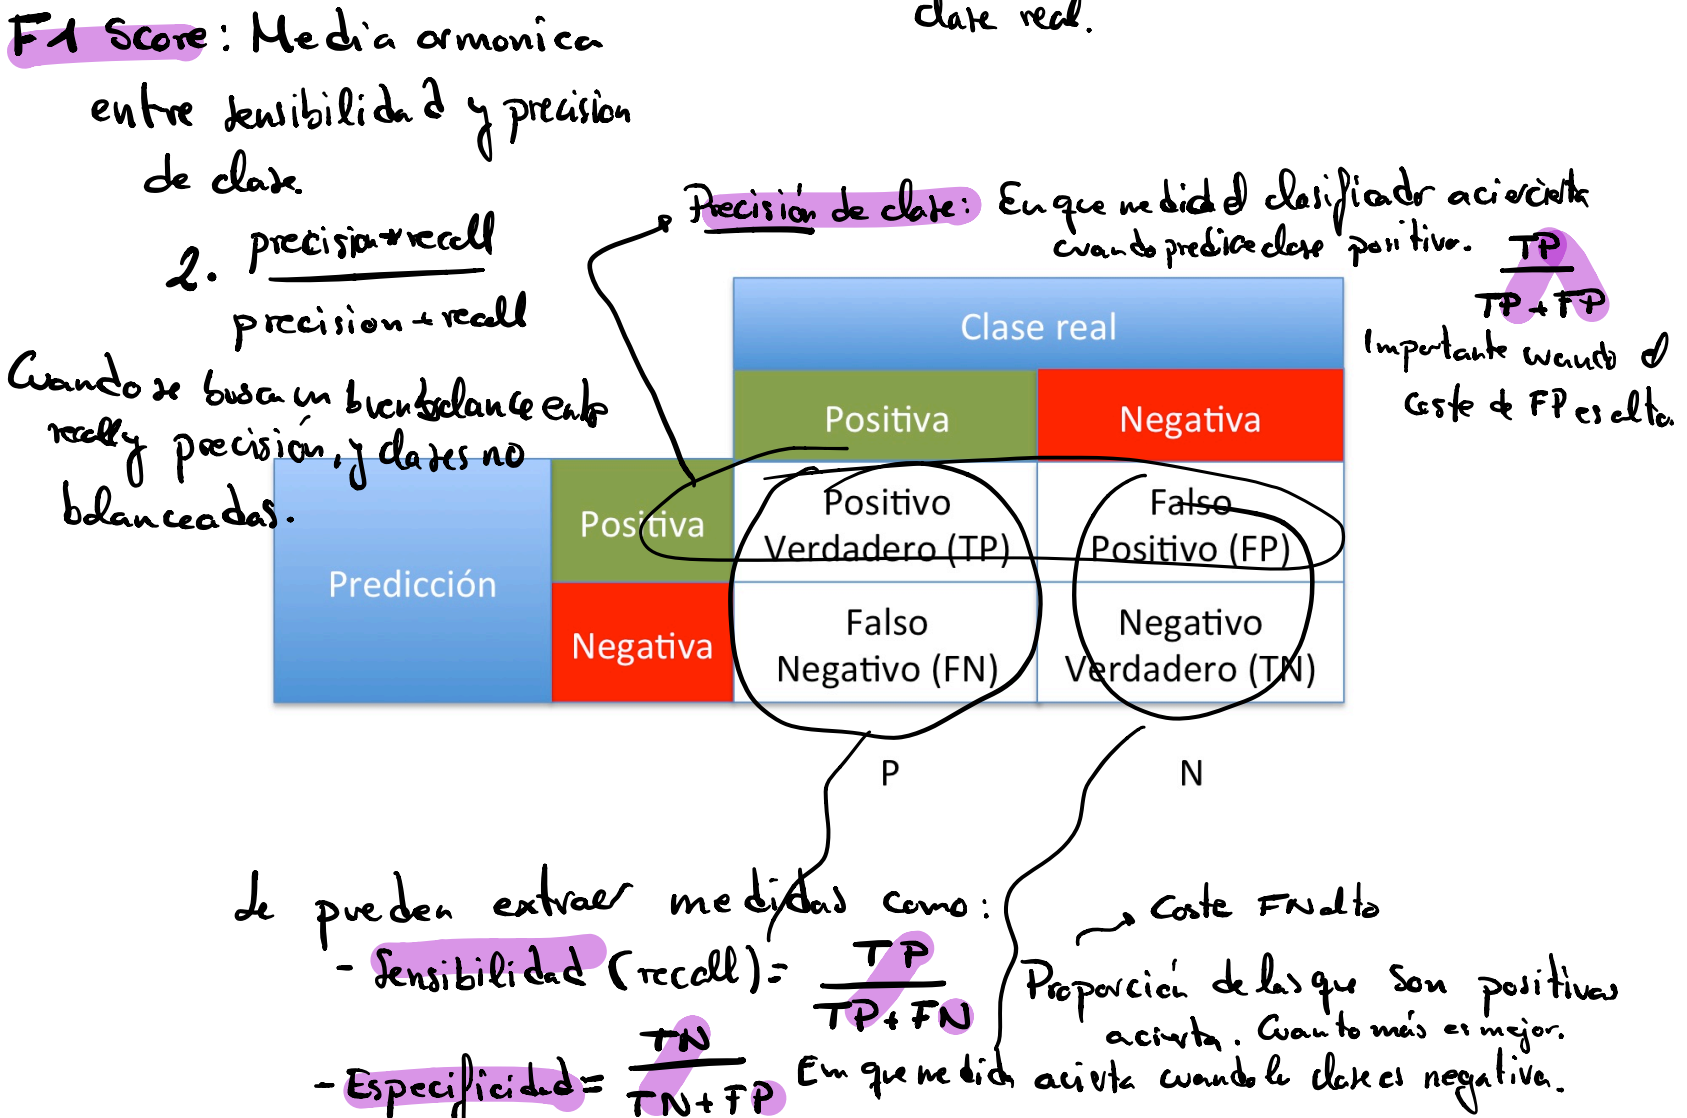
\includegraphics[scale=.2]{Untitled 11.png}}
\end{figure}

\(Accuracy= \frac {TP+TN}{TP+TP+FP+FN}\)

\(Sensibilidad(recall)= \frac {TP}{TP+FN}\) Proporción de las que son
positivas acierta. Cuanto más es mejor.

Cuando el coste de FN es alto.

\(Especificidad= \frac {TN}{TN+FP}\) En qué medida acierta cuando la
clase es negativa.

\(Tasa \space de\space falsos \space positivos=1-Especificidad= \frac {FP}{TN+FP}\)

\(Precision \space de \space clase= \frac {TP}{TP+FP}\) En qué medida el
clasificador acierta cuando predice clase positiva.

Importante cuando el coste FP es alto.

\(F1 \space score= 2\cdot \frac {precision \cdot recall}{precision +recall}\)
Medida armónica entre sensibilidad y precisión de clase.

Cuando se busca un buen balance entre recall y precisión de clase, y las
clases no balanceadas.
\newpage
\textbf{Espacio ROC:} Mide como de útil es un clasificador para
distinguir entre clases. Cuanto más cerca de la esquina superior
izquierda mejor, recoge más área y está más cerca del punto óptimo.
\begin{figure}[H]
	Ejemplo
	\ffigbox[\FBwidth]
	{\caption{Espacio ROC}}
	{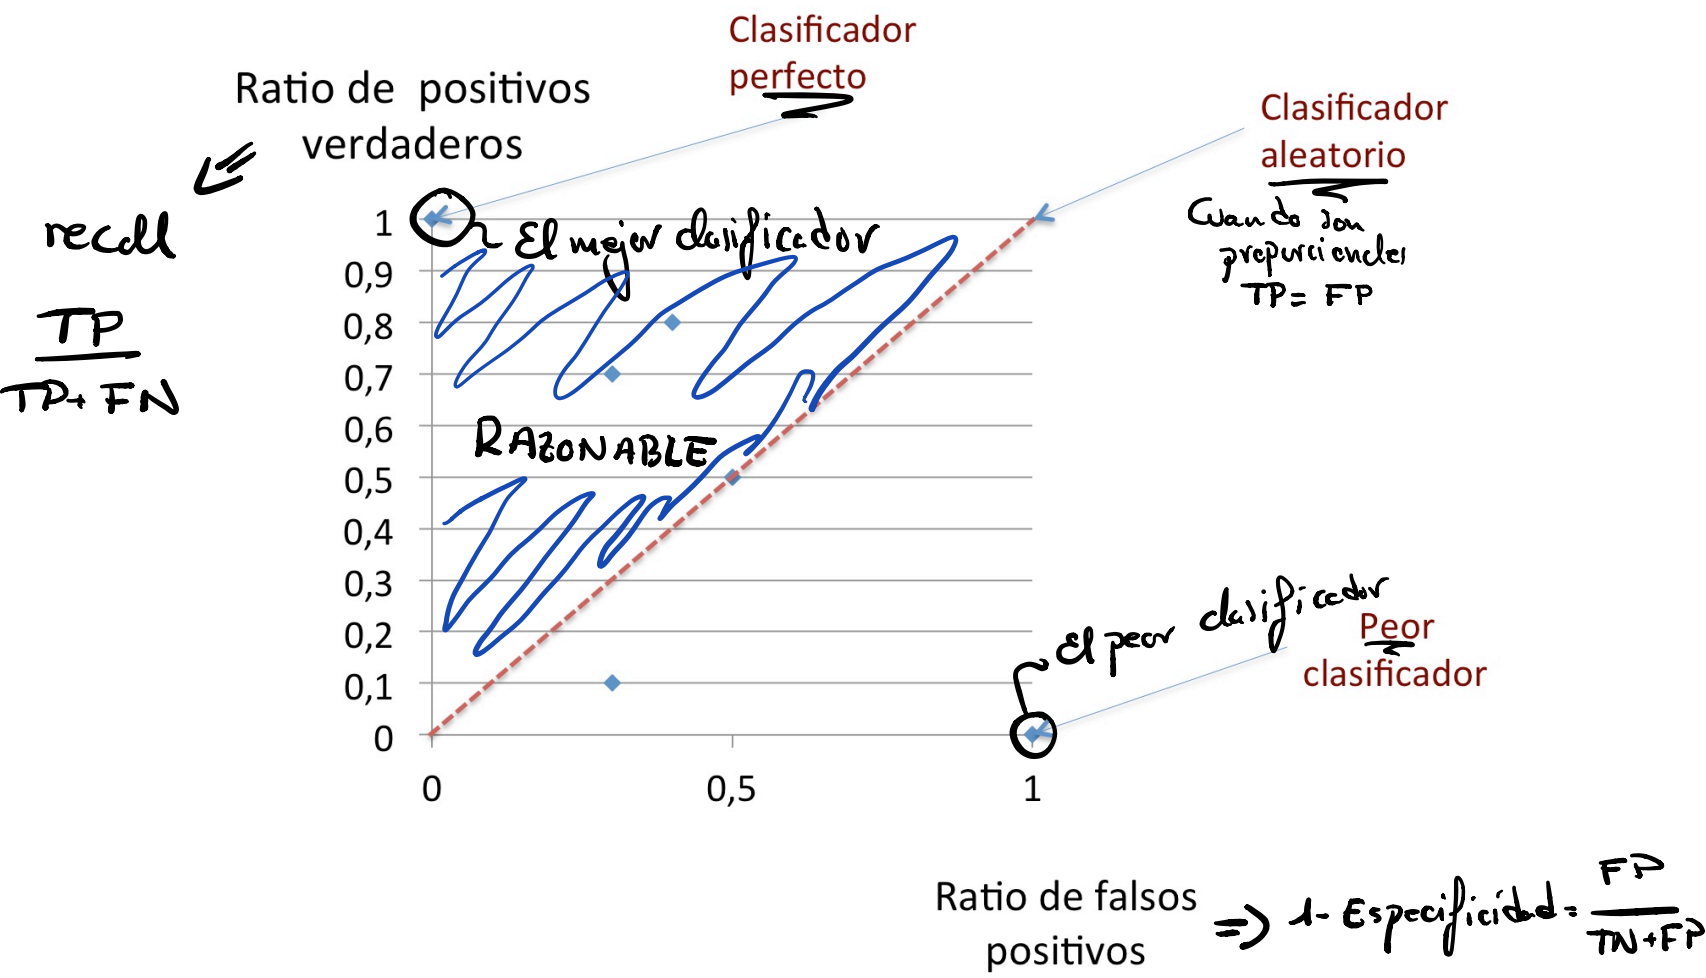
\includegraphics[scale=.2]{Untitled 12.png}}
\end{figure}
\textbf{Curva ROC}: Es una curva en el espacio ROC, en la que cada punto
de la recta representa un clasificador, el más cercano al punto óptimo
será el mejor, pero teniendo cuidado de los falsos positivos. Se define
un umbral a partir del cual se considera de clase positiva o negativa.
Los puntos son del tipo +0.8 +0.6.

Cuanto más Área por debajo de la curva mejor.

\begin{figure}[H]
	Ejemplo
	\ffigbox[\FBwidth]
	{\caption{Umbrales curvas ROC}}
	{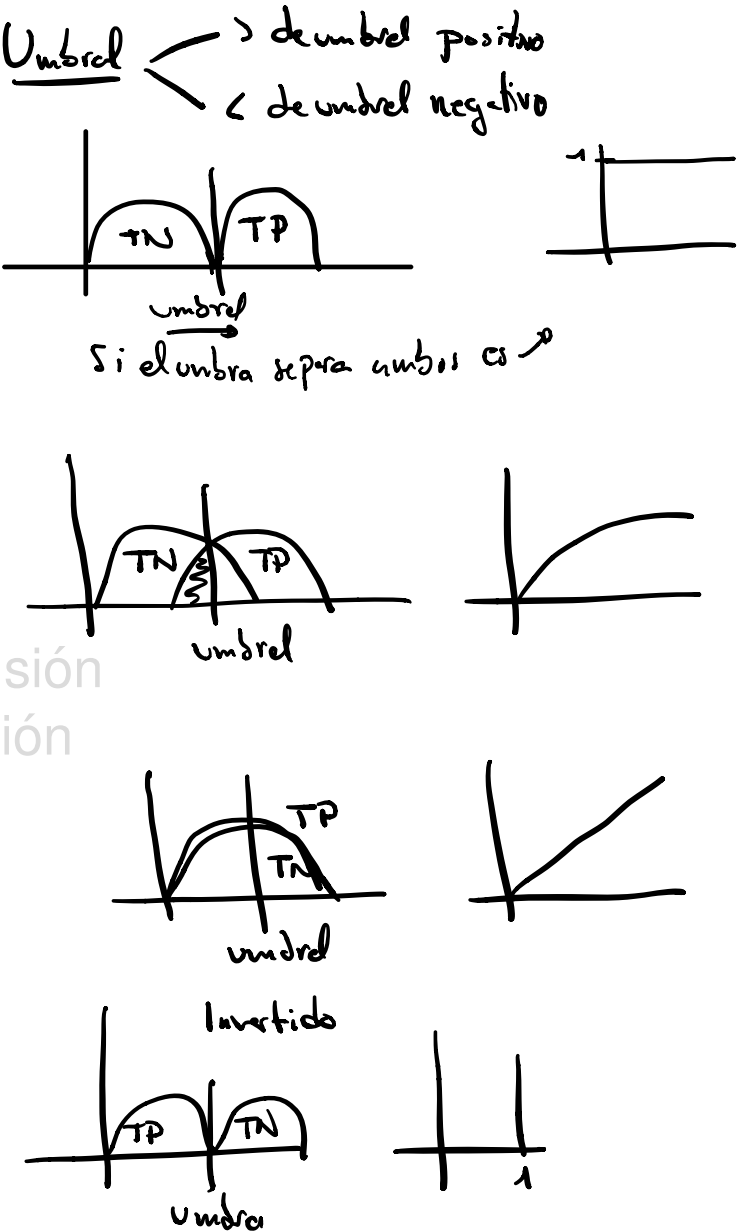
\includegraphics[scale=.2]{Untitled 13.png}}
\end{figure}

\section{Proceso de análisis de
datos}

Es un proceso iterativo, tras la última etapa se vuelve al principio.

\begin{enumerate}
\def\labelenumi{\arabic{enumi}.}
\item
  \textbf{Pre-procesamiento}.

  \begin{itemize}
  \item
    \textbf{Tratamiento de datos imperfectos:}

    \begin{itemize}
    
    \item
      \textbf{Reducción del ruido:} Mediante filtros que eliminan
      instancias clasificadas mal.
    \item
      \textbf{Valores desconocidos:} Eliminar instancias/atributos o
      asignar el valor más probable.
    \end{itemize}
  \item
    \textbf{Reducción de datos:} Reducir la variedad.

    \begin{itemize}
    \item
      \textbf{Normalización}: Valores entre 0 y 1.
    \item
      \textbf{Discretización}: En rangos.
    \item
      \textbf{Selección de instancias}: Aleatoriamente, los más
      parecidos entre sí, los más diferentes entre sí o según alguna
      distribución.
    \item
      \textbf{Selección de atributos:}

      \begin{itemize}
      \item
        Reducción de la dimensionalidad de los datos, mediante filtrado
        según algún criterio o seleccionando un subconjunto.
      \item
        \textbf{Búsqueda}: Cualquier técnica.
      \item
        \textbf{Evaluación}: Correlación, entropía, etc.
      \item
        \textbf{Criterio de parada:} Porcentaje, umbral, iteraciones,
        etc.
      \item
        \textbf{Técnicas de wrapper}: Se genera el modelo con todos los
        atributos, se evalúa el modelo y se ve el subconjunto de
        atributos mejores.
		\begin{figure}[H]
			Ejemplo
			\ffigbox[\FBwidth]
			{\caption{Técnicas de wrapper}}
			{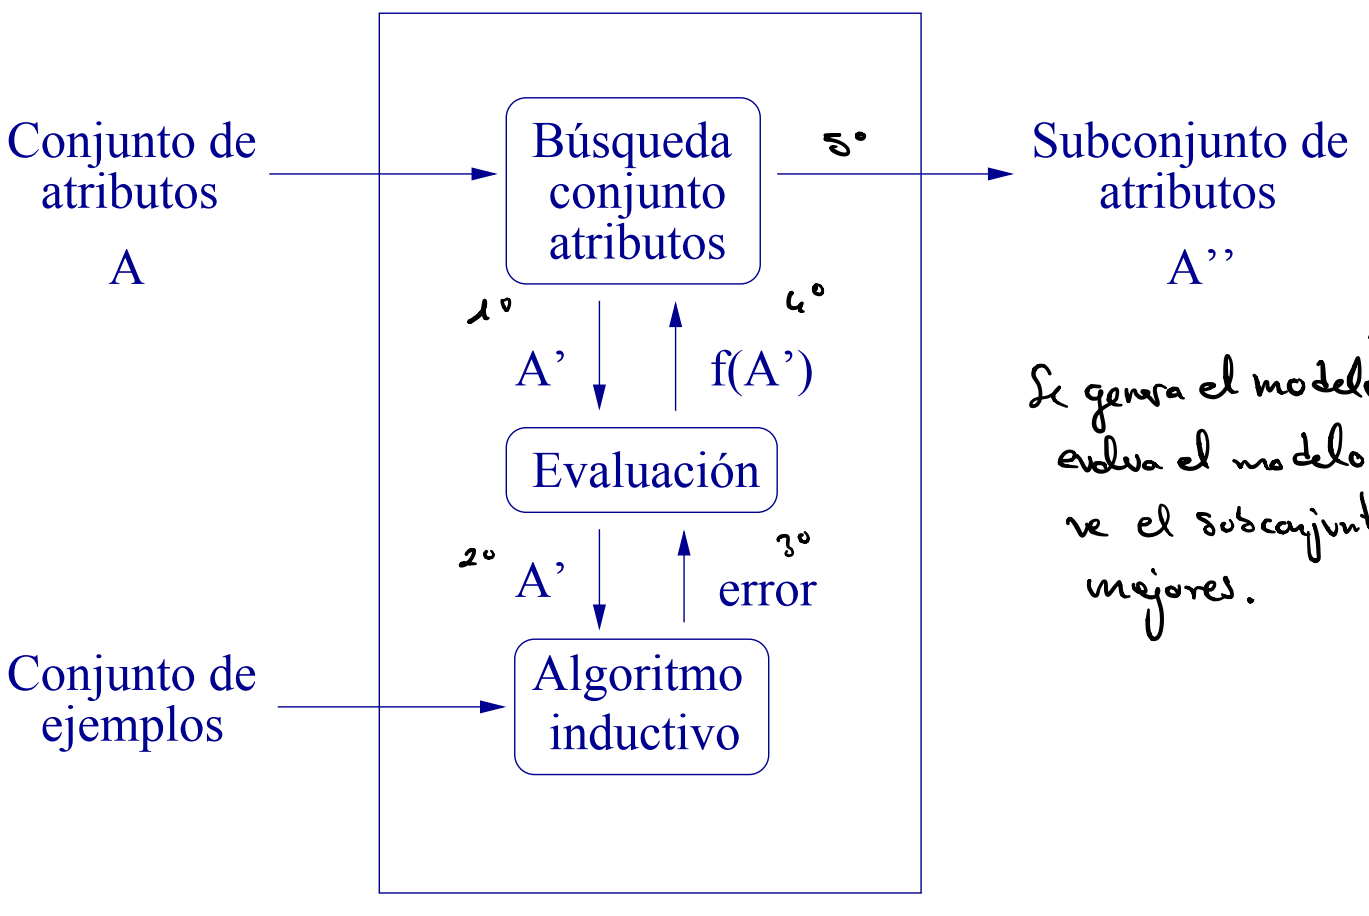
\includegraphics[scale=.2]{Untitled 14.png}}
		\end{figure}
      \item
        \textbf{Búsqueda en el espacio de estado de los conjuntos de
        atributos.}
		\begin{figure}[H]
			Ejemplo
			\ffigbox[\FBwidth]
			{\caption{Búsqueda por atributos}}
			{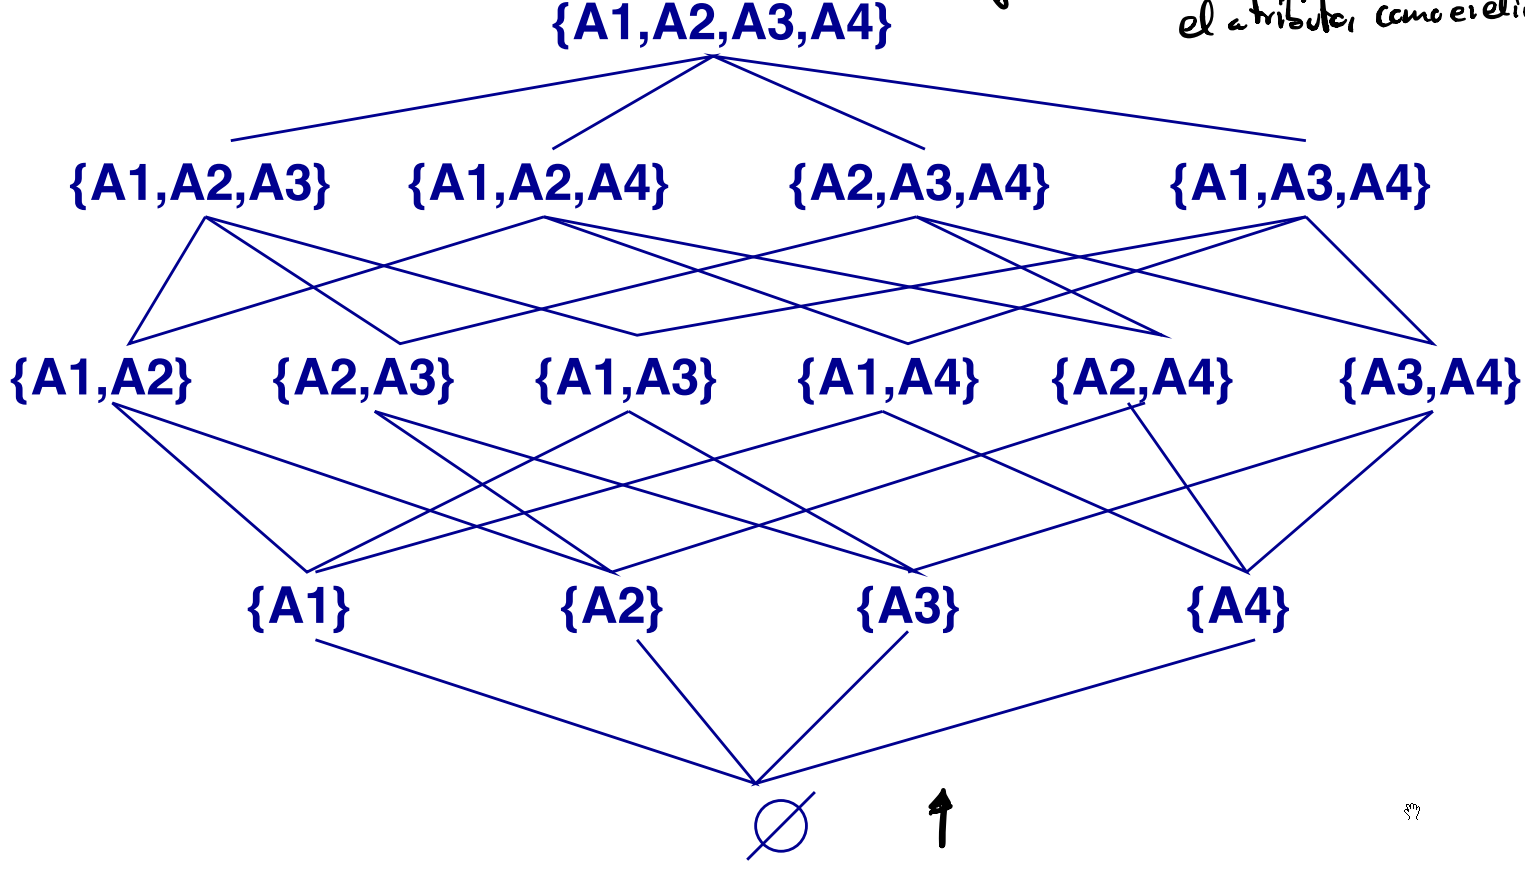
\includegraphics[scale=.2]{Untitled 15.png}}
		\end{figure}
        \begin{itemize}
        
        \item
          Se puede comenzar por el conjunto completo (por arriba) o por
          el conjunto vacío (por abajo).
        \item
          La búsqueda puede ser de cualquier tipo.
        \item
          La evaluación de cada nodo, que son subconjuntos de atributos,
          se realiza llamando al algoritmo inductivo seleccionado, una
          función de evaluación. Tras evaluar se opera.
        \end{itemize}
      \item
        \textbf{PCA (No lo usaremos):} Análisis de componentes
        principales. Es una solución algebraica, describe los datos en
        términos de nuevos atributos que no están correlados entre sí.
      \end{itemize}
    \item
      \textbf{Datos no balanceados:} Crear ejemplos sintéticos de la
      clase desbalanceada.
    \end{itemize}
  \end{itemize}
\item
  \textbf{Diseño}.

  \begin{itemize}
  
  \item
    Selección de algoritmo.
  \item
    Selección de parámetros.
  \end{itemize}
\item
  \textbf{Ejecución de algoritmo.}
\item
  \textbf{Post-proceso.}

  \begin{itemize}
  
  \item
    Análisis de resultados.
  \item
    Visualización.
  \end{itemize}
\end{enumerate}

\section{Aspectos avanzados}

\subsection{Sobreajuste
(overfitting)}

\begin{figure}[H]
	Ejemplo
	\ffigbox[\FBwidth]
	{\caption{Diagrama de sobreajuste}}
	{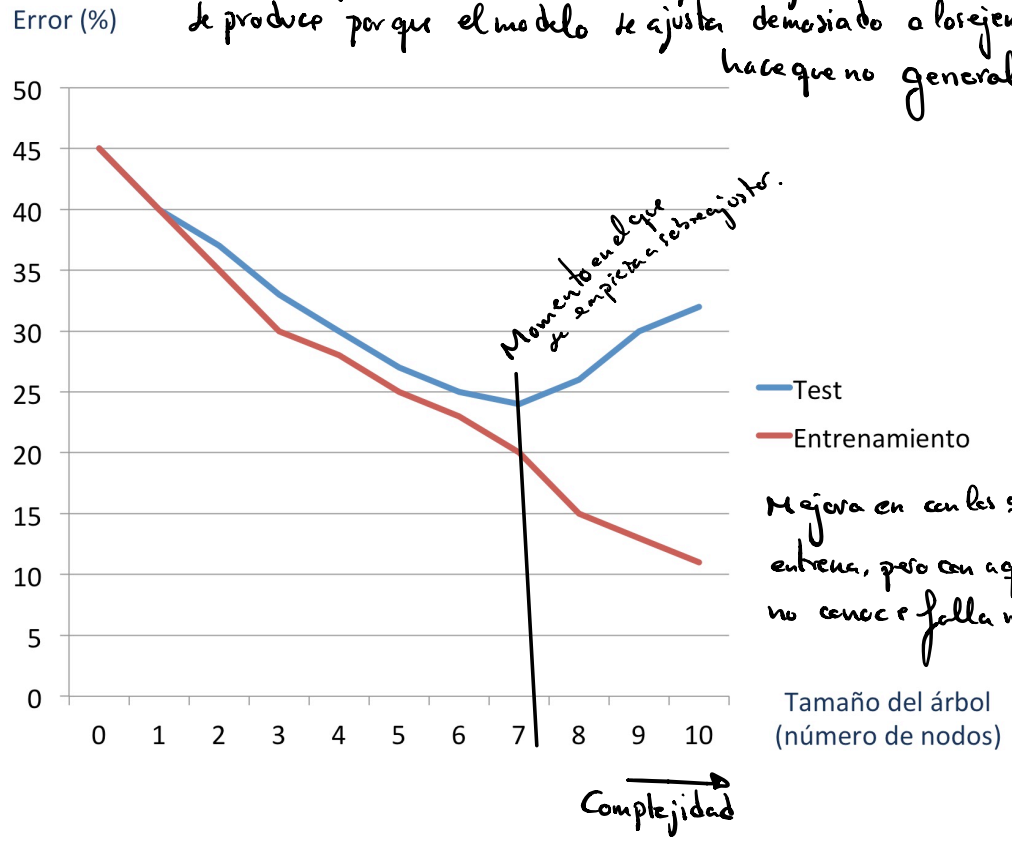
\includegraphics[scale=.2]{image-20210305195646416.png}}
\end{figure}

Fenómeno que se produce al hacer aprendizaje, porque \textbf{el modelo
se ajusta demasiado a los ejemplos, y eso hace que no generalice bien.}

Mejora con los que se entrena, pero con aquellas que no conoce falla
más.

Para evitar sobreajuste se debe generalizar, hay \textbf{2 métodos}:

\begin{itemize}
\item
  \textbf{Pre-poda}: Mientras se construye se poda.

  \begin{itemize}
  
  \item
    \textbf{Método de \(\chi^2\) (chi-cuadrado)}: Si en un nodo la
    diferencia entre clases no es significativa, no se divide, para con
    la mayoría. Muy conservador.
  \item
    \textbf{Mediante curvas de error}: Cross-validation. De esta manera
    podemos detectar el punto de inflexión, donde se empieza a producir
    overfitting (en el punto que se separan las curvas).
  \end{itemize}
\item
  \textbf{Post-poda}: Después de generar poda.

  \begin{itemize}
  \item
    \textbf{Eliminando subárboles}: Eliminando nodos del árbol empezando
    por las hojas, se evalúa el error tras eliminarlo, si no mejora
    probamos otro.

	\begin{figure}[H]
		\ffigbox[\FBwidth]
		{\caption{Arboles en Post-poda}}
		{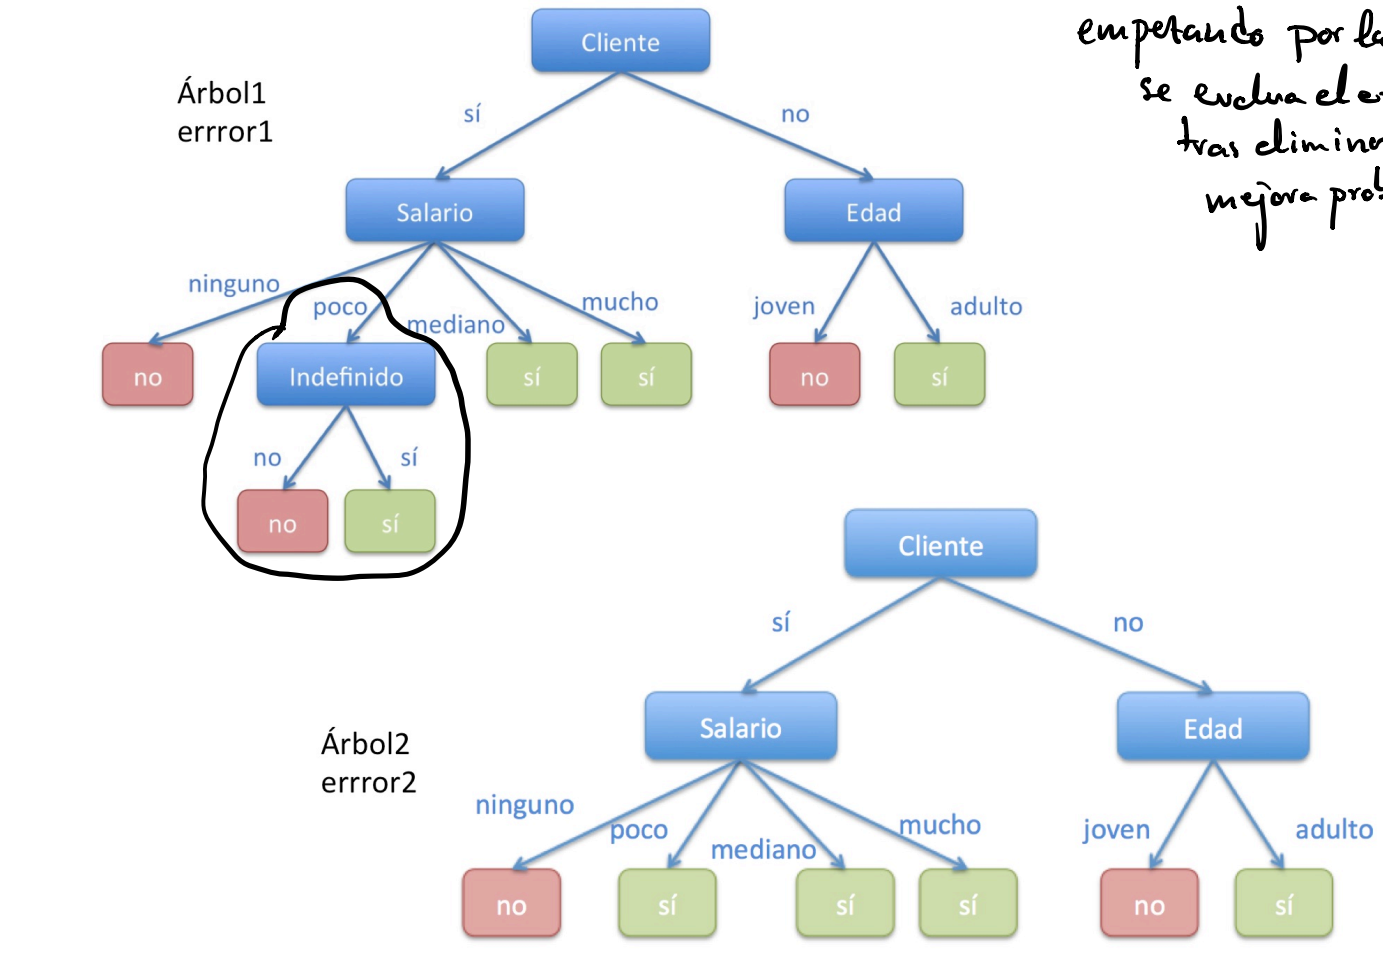
\includegraphics[scale=.2]{image-20210305200826542.png}}
	\end{figure}
  \item
    \textbf{Eliminando precondiciones o reglas}: Tras haberlo pasado a
    reglas, eliminamos condiciones o reglas completas. Tras la
    eliminación se calcula el error, si mejora, el modelo principal pasa
    a ser el que lo eliminó y se sigue probado. Si no se prueba otra
    condición o regla.
	\begin{figure}[H]
		\ffigbox[\FBwidth]
		{\caption{Eliminación de atributos/reglas Post-poda}}
		{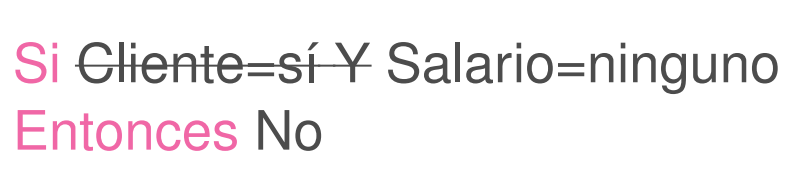
\includegraphics[scale=.2]{image-20210305201114245.png}
		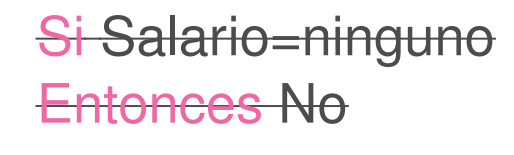
\includegraphics[scale=.2]{image-20210305201127523.png}}
	\end{figure}
  \end{itemize}
\end{itemize}

\subsection{Atributos con valores
continuos}
\begin{figure}[H]
	\ffigbox[\FBwidth]
	{\caption{Tratamiento de valores continuos}}
	{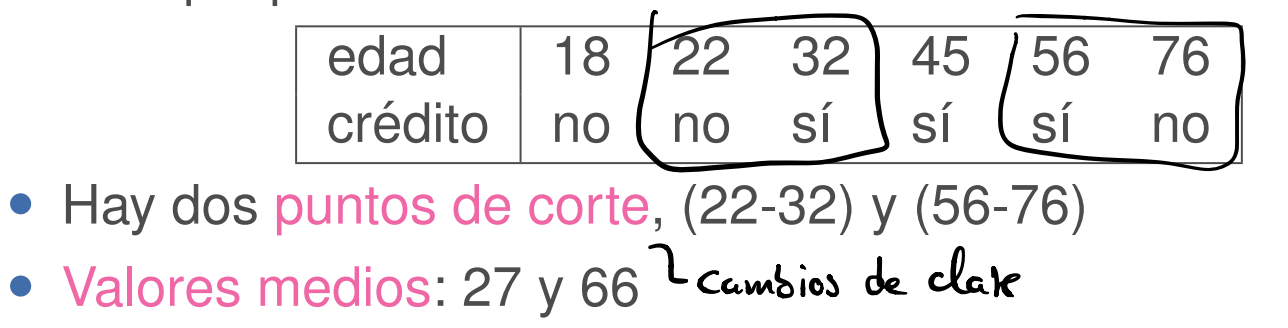
\includegraphics[scale=.2]{image-20210305201824512.png}}
\end{figure}

\begin{enumerate}
\def\labelenumi{\arabic{enumi}.}

\item
  Se \textbf{ordenan los valores del atributo}, y se especifica la clase
  a la que pertenecen.
\item
  Se \textbf{observan los puntos en los que pasa de una clase a otra} y
  se hace media con los puntos de corte.
\item
  Los \textbf{nodos de decisión se crean según:}

  \begin{itemize}
  
  \item
    Se trata como \textbf{atributo binario}: Se escoge \textbf{una sola
    regla de distinción} entre valores, el de mayor ganancia de
    información, que se eligen con los valores medios. Las reglas son del
    tipo atrib\textless punto1 o atrib\textless punto2.
  \item
    Se trata como \textbf{atributos multivaluado}: Se crean
    \textbf{tanto grupos como queramos}, lo más preciso es uno por cada
    intervalo de valores que tengan la misma clase.
  \end{itemize}
\end{enumerate}

\subsection{Atributos con muchos
valores}

\textbf{ID3 prefiere atributos con mayor número de valores.}

\textbf{Problema}: Que cada uno puede tener un valor único, y no se
podrá usar para clasificar.

\textbf{Alternativas}:

\begin{itemize}

\item
  Por cada valor v del atributo A, se puede crear un atributo binario,
  de si es atributo toma ese valor o no.
\item
  \textbf{Razón de ganancia (GainRatio, GR)}: Ganancia calculada como la
  ganancia partido por una penalización por el número de valores del
  atributos.
  $$
  GR(S,A)= \frac {G(S,A)=max Entropia(S)-EntropiaAtrib(S,A)}{Split\_Information(S,A)=-\sum_{c\in valores(A)} \frac {|S_v|}{S} \cdot log_2(\frac {S_x}{S})}
  $$
\item
  \textbf{Split\_Information(S,A)}: Entropía de S con respecto de A.
  $$
  Split\_Information(S,A)=-\sum_{c\in valores(A)} \frac {|S_v|}{S} \cdot log_2(\frac {S_x}{S}) 
  $$
\end{itemize}

\subsection{Atributos con costes
variables}

Como podrían ser pruebas médicas caras, obtener los ejemplos es caro.
\textbf{Consiste en penalizar la entropía de los atributos con coste
variable.}

\(\frac {G(S,A)}{unidad \space de \space coste(A)} o \frac {G(S,A)}{unidad \space de \space coste(A)^2}\)

\section{Otras alternativas a ID3}

\textbf{Clasificadores débiles:}

\begin{itemize}

\item
  \textbf{ZeroR}: En clasificación, dará siempre la \textbf{clase más
  frecuente}, la moda de la clase. En regresión, devuelve la media.
\item
  \textbf{OneR}: Construye un conjunto de \textbf{reglas de decisión con
  un solo atributo}. Se elige aquel atributo con menor error, para cada
  valor del atributo se crea una regla, donde el valor que toma es el
  más frecuente.
\end{itemize}

\section{Implementaciones}

\begin{description}
	\item[ID3, 1986]
	\item[C4.5, 1993] Sucesor de ID3, atributos numéricos, conversación a reglas, poda.
	\item[C5.0] Versión comercial.
	\item[J4.8] Implementación JAVA de C4.5.
\end{description}

\chapter{TEMA 3. Regresión}
\begin{figure}[H]
	\ffigbox[\FBwidth]
	{\caption{Ejemplo instancias de Regresión}}
	{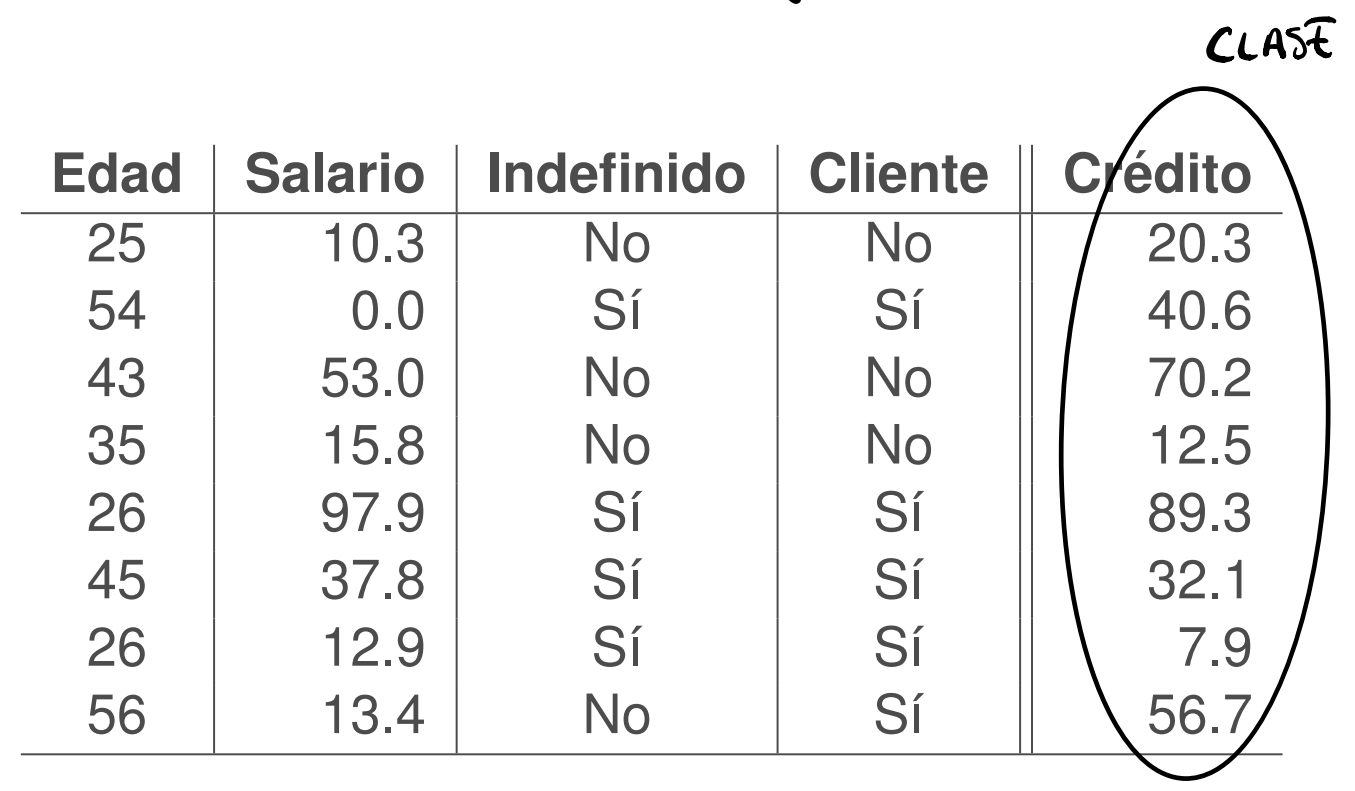
\includegraphics[scale=.2]{image-20210305210244509.png}}
\end{figure}
La clase en regresión es numérica.

\section{Regresión como
clasificación}

Discretizando la clase, pero se pierde información y hay que elegir un
método de discretización.

\textbf{Soluciones}:

\begin{itemize}

\item
  \textbf{Discretización de clase.}
\item
  \textbf{Discretización fija.}
\item
  \textbf{Discretización dinámica.}
\end{itemize}

\section{Función de regresión}
\begin{figure}[H]
	\ffigbox[\FBwidth]
	{\caption{Ejemplo Regresión Lineal}}
	{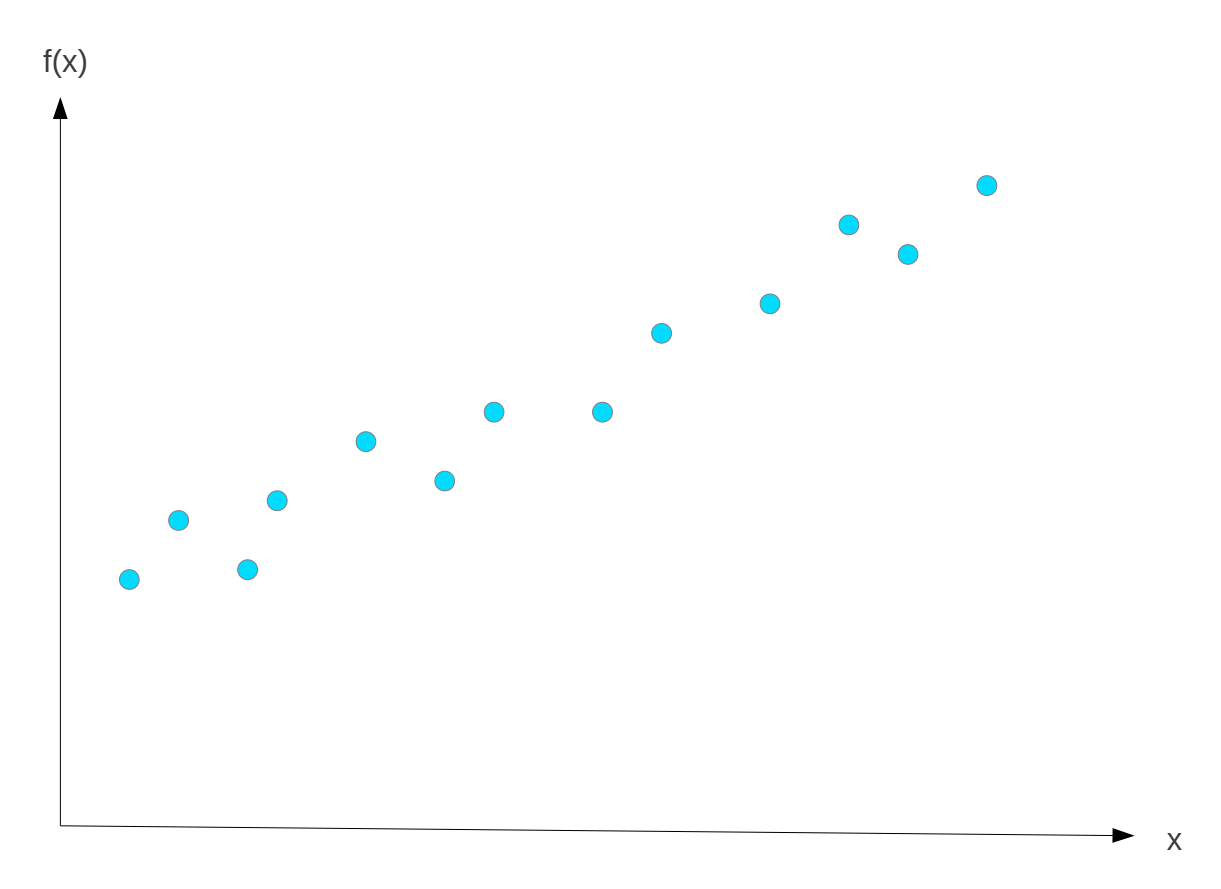
\includegraphics[scale=.15]{image-20210305211354068.png}
	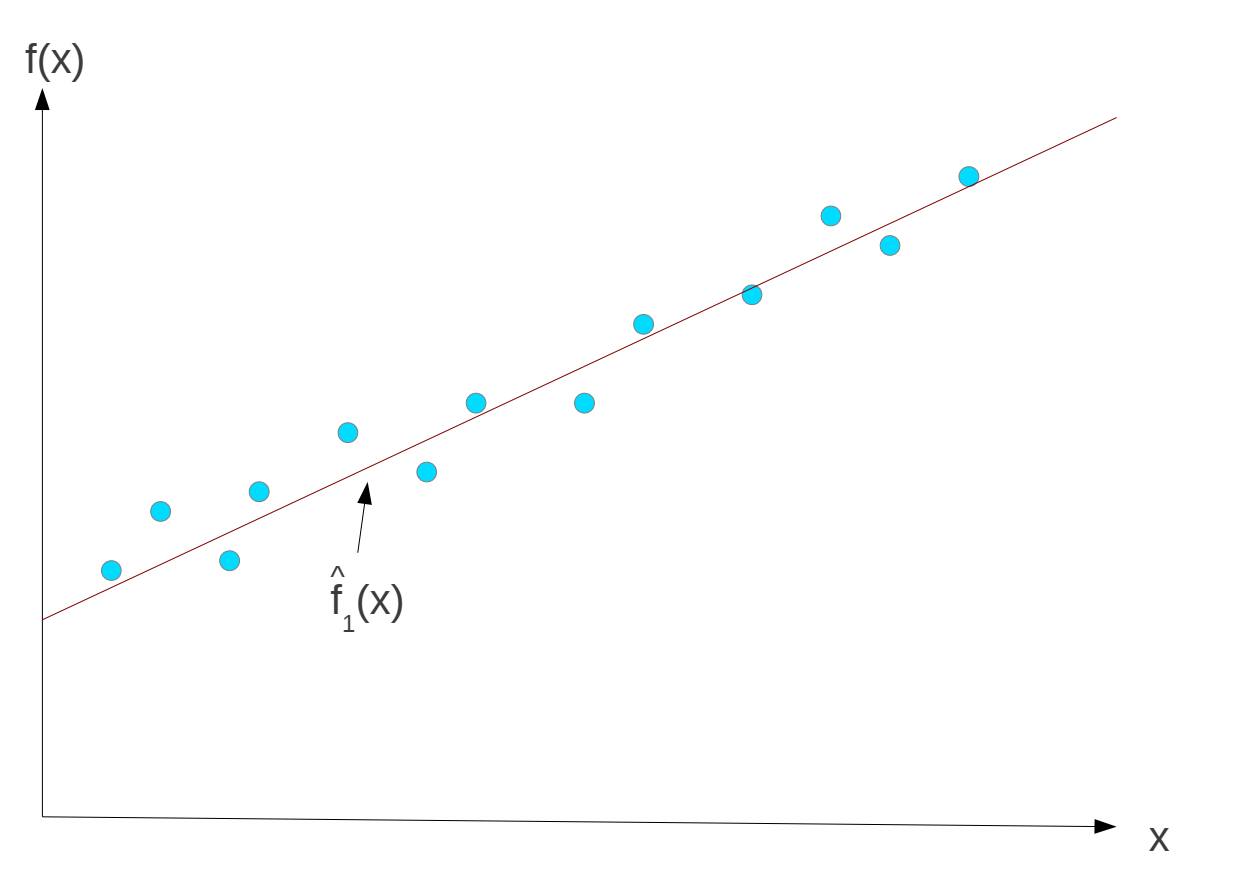
\includegraphics[scale=.15]{image-20210305211454026.png}}
\end{figure}

\subsection{Regresión lineal}

Hallar una \textbf{función que se ajuste lo mejor posible a la nube de
puntos}. En el caso de la \textbf{lineal es una recta.}

Aproximar una función \(f(x)\) que no tiene por qué ser lineal en
regresión, con una función
\textbf{\(\hat{f}(x)= w_0 + w_1a_1(x)+ w_2a_2(x)+ ...+ w_na_n(x)\)}
donde

\begin{itemize}

\item
  \(a_i\) denota el \textbf{atributo} i-ésimo del ejemplo x.
\item
  \(w_i\) \textbf{peso} del atributo
\end{itemize}

\textbf{Objetivo}: Encontrar aquellos \(w_i\) que minimicen el error
entre la función clase y el valor de la aproximación.

Equivalente a \textbf{minimizar el error cuadrático sobre el conjunto de
entrenamiento total,} C: \(E= \sum _{c \in C} (f(x)-\hat{f}(x))^2\) Lo
que queremos es minimizar.

\subsection{Error de Regresión}

La \textbf{suma de todas las diferencias de los valores de la función y
su aproximación}. Buscamos aquella aproximación que minimice E.
\begin{figure}[H]
	\ffigbox[\FBwidth]
	{\caption{Ejemplo de error en Regresión Lineal}}
	{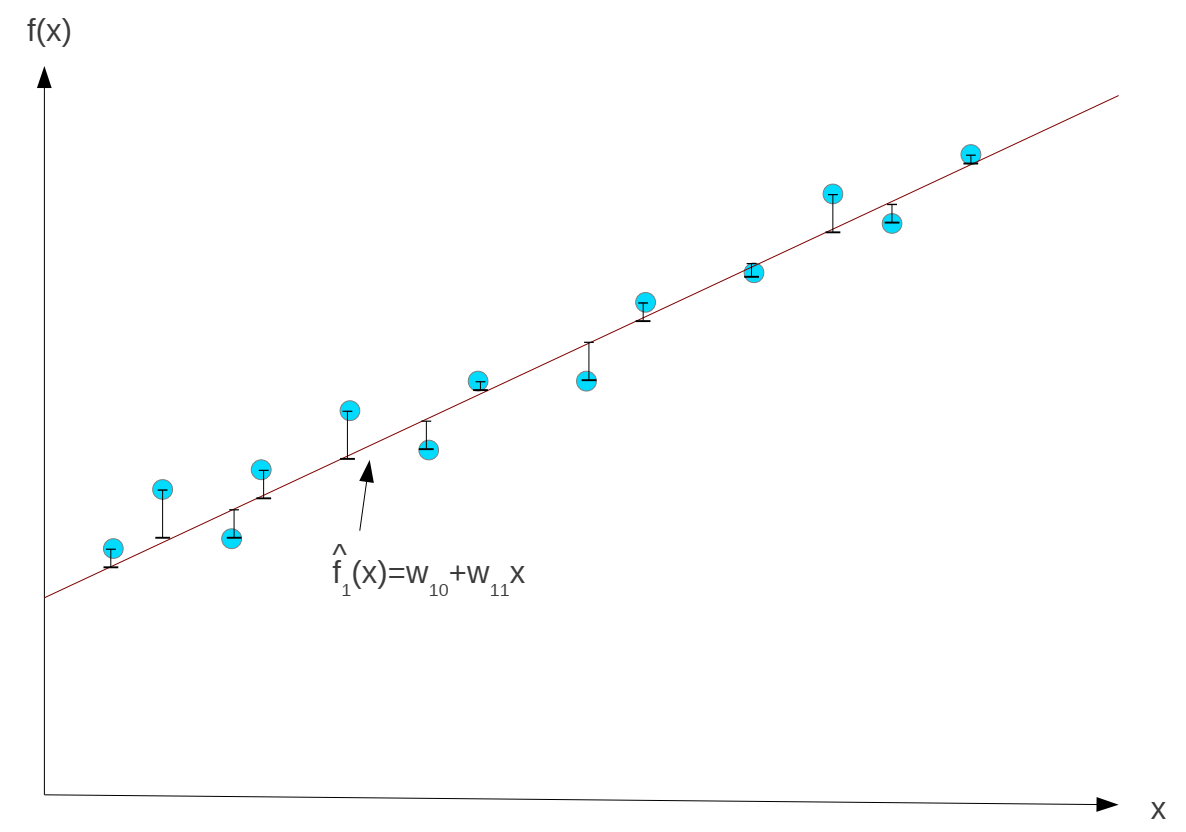
\includegraphics[scale=.10]{image-20210305212854142.png}}
\end{figure}

\subsubsection{Minimizando el error}

\textbf{El problema de definir la función se traslada a un problema de
definir el vector de pesos w.} Se debe encontrar el vector \(\vec{w}\)
que minimice la función de error, problema de búsqueda en el espacio de
pesos.

\textbf{Aproximación}: Descenso de gradiente.

\subsection{Descenso de gradiente}
\begin{figure}[H]
	\ffigbox[\FBwidth]
	{\caption{Diagrama de Descenso de Gradiente}}
	{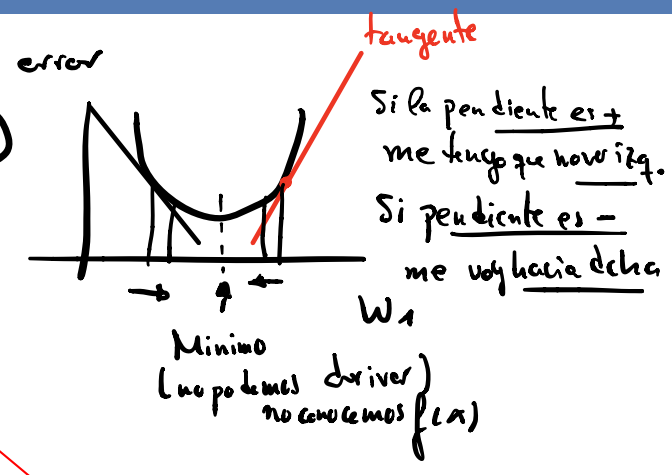
\includegraphics[scale=.3]{image-20210305214445428.png}}
\end{figure}
Sobre la función de errores por variable \textbf{vamos calculando la
tangente y desplazando los valores de los pesos}.

\begin{itemize}

\item
  Consisten en movernos poco a poco en los pesos, para no pasarnos, y se
  parte de pesos aleatorios.
\item
  Si la \textbf{tangente} tiene pendiente \textbf{positiva}, nos
  desplazamos a la \textbf{izquierda}.
\item
  Si la \textbf{tangente} tiene pendiente \textbf{negativa}, vamos a la
  \textbf{derecha}.
\end{itemize}

\textbf{Gradiente del error respecto a w:} Derivada parcial de la
función de error de cada uno de los pesos.
\(\nabla E[\vec{w}] \equiv\left[\frac{\partial E}{\partial w_{0}}, \frac{\partial E}{\partial w_{1}}, \cdots \frac{\partial E}{\partial w_{n}}\right]\)

\textbf{Regla de entrenamiento:}
\(\Delta \vec{w}=-\eta \nabla E[\vec{w}]\)

\textbf{Derivada del error:}
\(\frac{\partial E}{\partial w_{i}}=\sum_{e}\left(t_{e}-o_{e}\right)\left(-x_{i, e}\right)\)

\begin{itemize}

\item
  \(t_e\): Valor \textbf{verdadero} para la instancia e.
\item
  \(o_e\): Valor de \textbf{salida del modelo} para la instancia e.
\item
  \(x_{i,e}\): Valor del \textbf{atributo} a para la instancia e.
\end{itemize}
\newpage
\textbf{Procedimiento: Descenso de Gradiente(C,n)}

\begin{itemize}

\item
  C conjunto de ejemplo de entrenamiento. n tasa de aprendizaje cuando
  salta.
\end{itemize}

\begin{figure}[H]
	\ffigbox[\FBwidth]
	{\caption{Algoritmo de Descenso de Gradiente}}
	{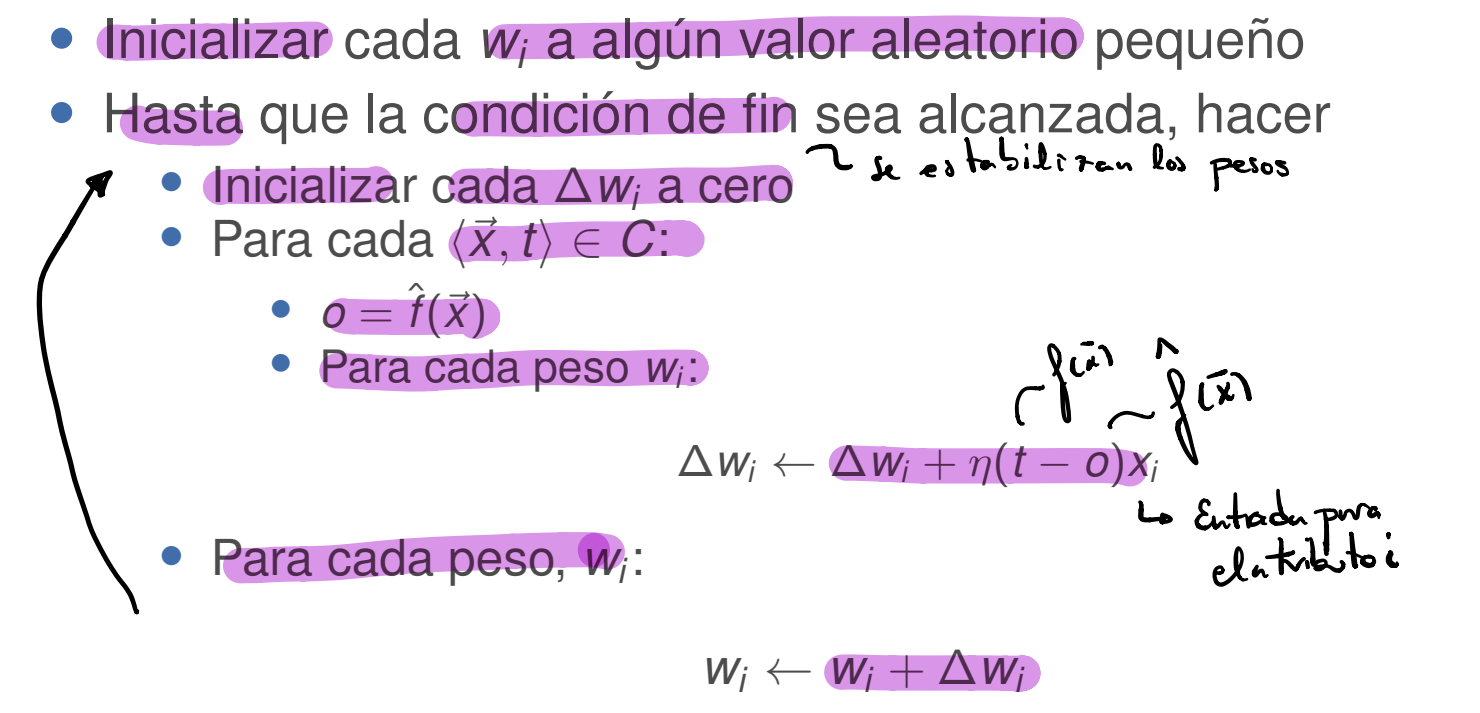
\includegraphics[scale=.2]{image-20210305224415026.png}}
\end{figure}

\subsection{Regresión no lineal}

Cuando usamos este tipo de funciones hay que tener \textbf{cuidado}, la
evaluación se debe realizar con ejemplos de un conjunto distinto al de
entrenamiento, porque la función no lineal se puede ajustar muy bien a
esos, pero no al resto.

Esta función es más difícil de generar.

\section{Regresión paramétrica}

Elegir una función lineal, logística o cualquier tipo, para que se
ajuste.

El modelo o predictor adopta una forma predeterminada.

Regresión lineal es regresión paramétrica. También se puede hacer
regresión no lineal paramétrica, función logística, polinómica, etc.

\section{Arboles de regresión}

Regresión no lineal y no paramétrica.

\section{M5}

\textbf{M5 es una variación de CART}, las hojas son valores numéricos y
elige aquel atributo que maximice la reducción esperada en varianza.

\textbf{Estrategia}: Se divide el espacio en partes y hace regresión
lineal por partes, no global.

\textbf{Algoritmo}: Parecido a ID3, pero en este caso se trata de
reducir la variación interna de los valores de la clase de cada
subconjunto.

\begin{itemize}
\item
  Elige aquel atributo que maximice la reducción del error (en vez de
  entropía o desviación típica). Nos quedamos con la menor media de
  desviaciones.

  \(\Delta \operatorname{error}(S, A)=\operatorname{sd}(S)-\sum_{v \in \text { valoresTestNodo }(A)} \frac{\left|S_{A=v}\right|}{|S|} \times \operatorname{sd}\left(S_{A=v}\right)\)

  \begin{itemize}
  
  \item
    \textbf{S} conjunto de ejemplos en el nodo a dividir.
  \item
    \textbf{\(S_{A=v}\)} Ejemplos con valor v en el atributo A.
  \item
    \textbf{sd(S)} Desviación típica de los valores de la clase para los
    ejemplos en S.
  \end{itemize}
\end{itemize}

\textbf{Criterio de parada}: Pocos ejemplos o poca variación de los
valores (desviación típica pequeña)

\textbf{Hojas}: Se calcula un modelo lineal y se utiliza regresión
estándar.

\textbf{Salida}: En las hojas tiene funciones de regresión, en los nodos
no hoja se tienen atributos acotados \textless. Cada nodo tiene un
conjunto de entrenamiento y se hace su regresión lineal.

\begin{figure}[H]
	\ffigbox[\FBwidth]
	{\caption{Diagramas M5}}
	{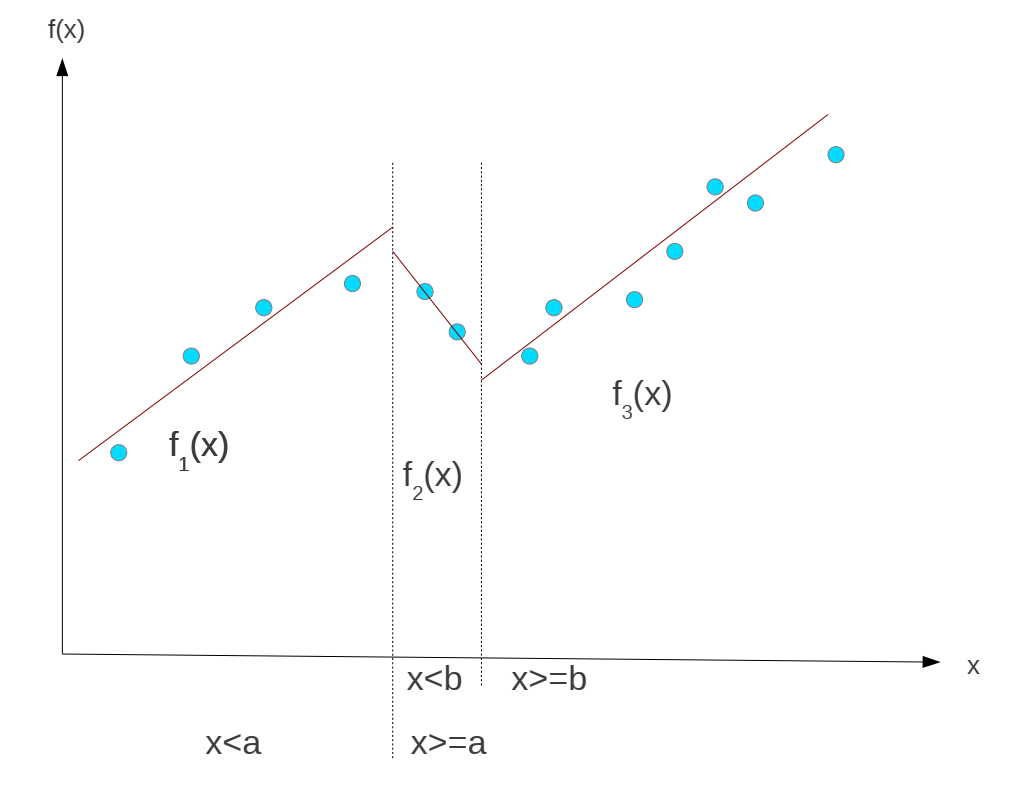
\includegraphics[scale=.2]{image-20210305230339091.png}
	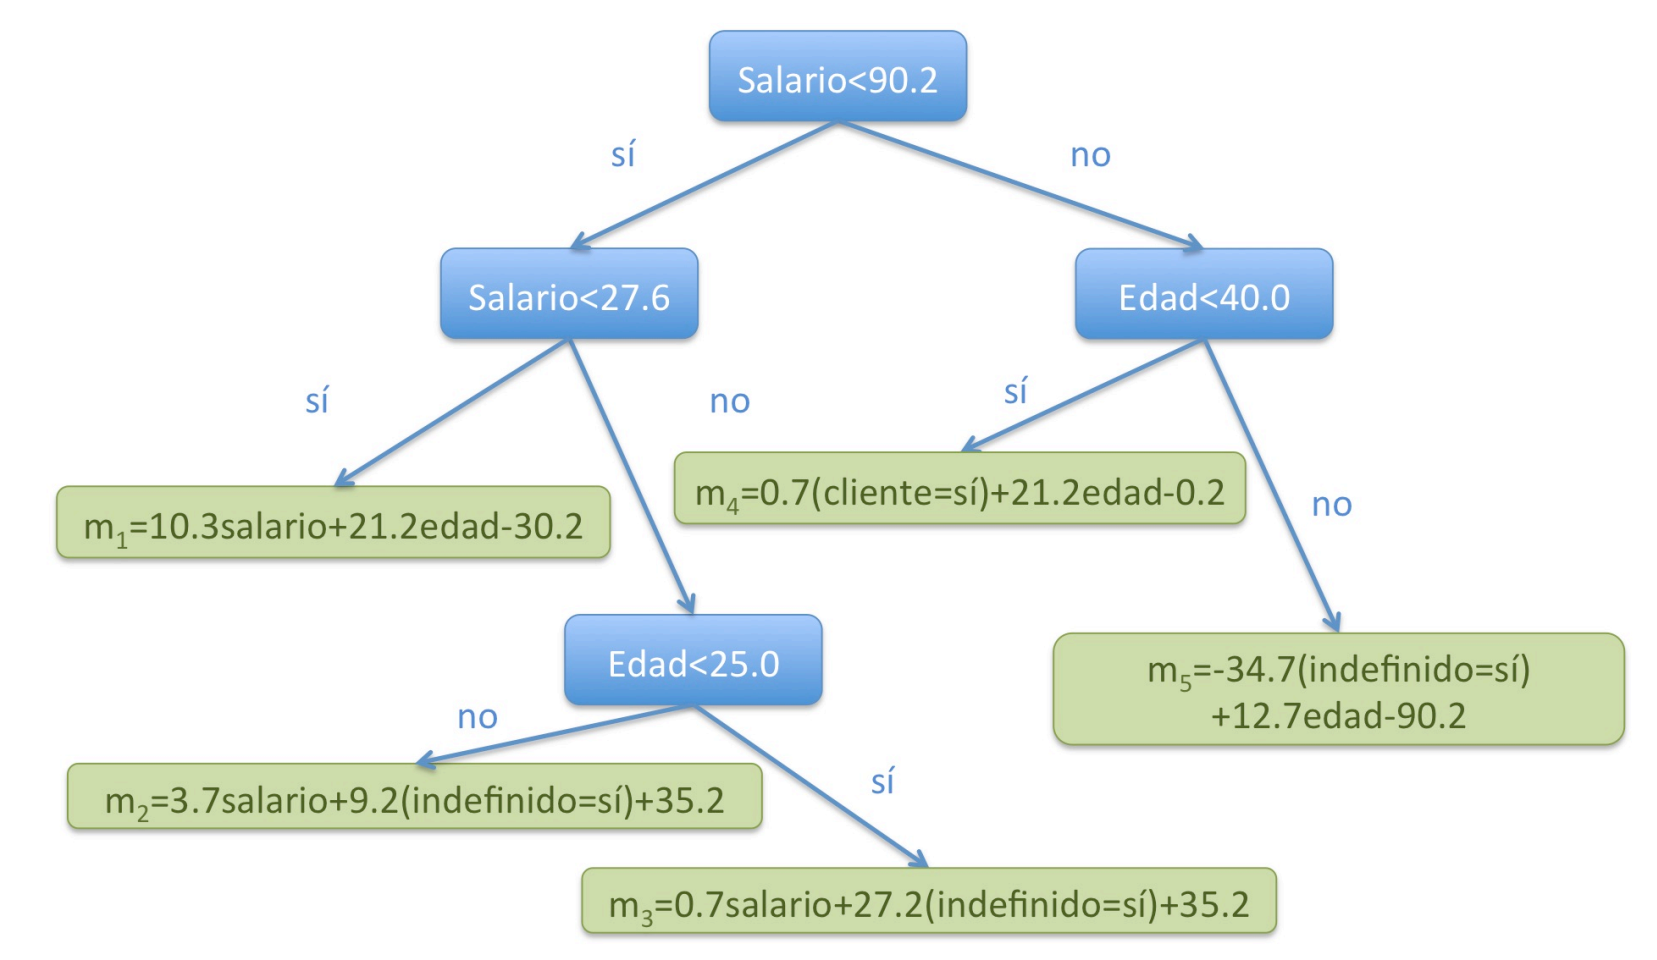
\includegraphics[scale=.15]{image-20210305230601935.png}}
\end{figure}
En los árboles de regresión, los nodos hoja tienen modelos lineales y
para llegar a esos nodos se usa como heurística es la Desviación típica
(cuanto menor mejor), que se calcula haciendo una media ponderada
(\(S_{S=si}\cdot\frac {|S_{S=si}|}{|S|}\)) de las desviaciones típicas
de cada uno de los conjuntos resultantes.

Tras la construcción del árbol hay un proceso de poda, que consiste en
Simplificar los modelos lineales de las hojas, Simplificar el árbol para
que sea más pequeño y por último el Suavizado.
\newpage
\section{Poda}

\textbf{Paso 0}: Antes de realizar la poda se crean modelos lineales de los nodos
intermedios, que se utilizaran para ver si se pueden simplificar los
subárboles por ese modelo del nodo intermedio. Para estos modelos se
usan solo los atributos que aparecen en el subárbol.

\begin{figure}[H]
	\ffigbox[\FBwidth]
	{\caption{Generación de modelos de nodos intermedios}}
	{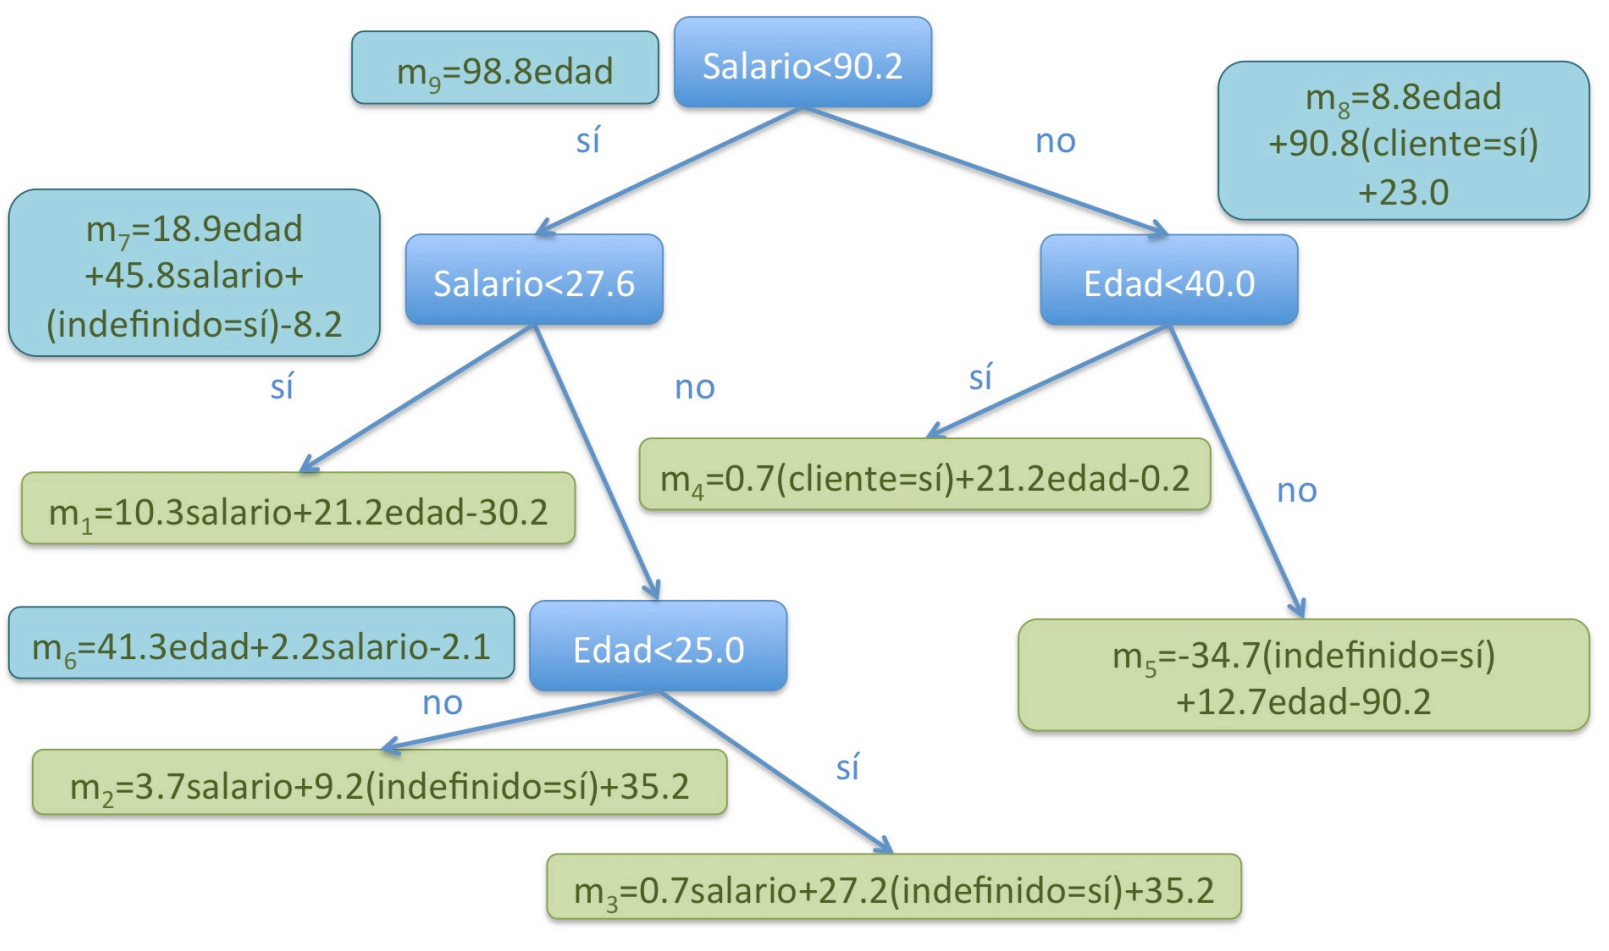
\includegraphics[scale=.15]{image-20210312090434196.png}}
\end{figure}

Para decidir si simplificamos por un modelo lineal necesitamos una
medida del error. Si el modelo lineal proporciona menor error con
respecto al subárbol podemos simplificarlo utilizando el modelo.

La medida de error que empleamos es el \textbf{Error absoluto medio},
que es la media de error al clasificar las instancias el subconjunto de
instancias de entrenamiento del subárbol. Se calcula como $residuo(T) = \frac 1 n \sum _{i \in T} ||f(i)- \hat{f}(i)||$, dado un
subárbol con un subconjunto de n instancias de entrenamiento T.

El residuo subestima el error en instancias nuevas (que no ha visto
nunca), para solucionar esto se multiplica por
\(\alpha = \frac {n+v}{n-v}\). Tal que n es el número de ejemplos del
subárbol y v el número de atributos del modelo.

Por lo que el error aumenta cuando hay muchos parámetros o hay pocas
instancias.

\textbf{Formula del error:}
\(error\_estimado(T) = \alpha \times residuo(T)\) Es una proporción del
residuo.

\begin{enumerate}
\def\labelenumi{\arabic{enumi}.}
\item
  \textbf{Simplificación de los modelos lineales} (Busca eliminar
  atributos)

  Se realiza en cada modelo lineal. Se eliminan atributos, que se
  seleccionan utilizando escalada para reducir el error estimado. En el
  extremo, deja solo una constante, como termino independiente.

  \(M= 0.25a_1+0.12a_2+300a_5-40 \Rightarrow M=0.12a_2+300a_5-40\)
\item
\textbf{Simplificación del subárbol} (Busca eliminar subárboles por modelo
  lineales)

  Cada nodo interno del árbol tiene un modelo lineal simplificado y un
  modelo subárbol, y se elige aquel que minimice el error estimado. Si
  el modelo da mejor resultado, se sustituye el subárbol por el nodo del
  modelo.
\item
  \textbf{Suavizar el árbol}

  Algunos trabajos se ha comprobado que realizar un suavizado mejora la
  predicción final, dado que lea predicción en cada nodo puede variar
  mucho. Lo que hace es en lugar de devolver la predicción del modelo en
  el nodo hoja. se consideran también los modelos en los nodos
  intermedios entre el nodo hoja y el nodo raíz.
\end{enumerate}

\chapter{TEMA 4. Resumen otras técnicas}

\section{Aprendizaje Bayesiano}

Funcionan bien en la clasificación de textos, text mining. Permite
recibir los datos de manera incremental y va creciendo el modelo.

\subsection{Hipótesis más probable
(MAP)}

Se busca la hipótesis que explique mejor los datos.
\[P(h_i/E)= \frac {P(E/h_i)P(h_i)}{P(E)}\]

Es aquella que \(\arg \max P(h_i/E)\) o $\arg \max P(E/h_i) $.
Cogemos el \(h_i\) más probable, pero puede haber otros muchos modelos
que dicen que no y que habría que considerar, entonces lo que queremos
es la clase más probable para esos datos.

\subsection{Clasificación más
probable}

Probabilidad de la clase C dados los ejemplos E:
\(P(C/E) = \sum _{h_i \in H} P(C/h_i) \cdot P(h_i/E)\)

A esto se le llama \textbf{Clasificador Bayesiano Optimo}, en la
practica el tamaño de H hace que sea imposible, además no tenemos un
modelo como tal si no la probabilidad de la clase más probable para esos
datos.

\subsection{Naïve Bayes}

\(\arg \max P(C/a_1, ...,a_n)= \arg \max _{c \in C} \frac {P(a_1, ...,a_n/C)P(C)}{P(a_1, ...,a_n)}=\arg \max_{c \in C} P(a_1, ...,a_n/C)P(C)\)

Podemos quitar el denominador porque todas las clases se evalúan con los
mismos atributos. Y \(P(a_1, ...,a_n/C)\) es muy complejo de calcular,
exponencial, se necesitaría una tabla de todas las combinaciones.

Para evitar esta complejidad se hace una simplificación, \textbf{se
asume que los valores de los atributos una vez se conoce la clase son
condicionalmente independientes}, lo que quiere decir que se puede
calcular como un producto.
\(P(a_1, ...,a_n/C) = P(a_1/C) \cdot P(a_2/C) \cdot ... \cdot P(a_n/C)\).
El problema es que ahora no es una aproximación y no un clasificador
bayesiano óptimo. \textbf{Suele funcionar bastante bien} esta
aproximación.

\(P(c=c_1)= \frac {n\_casos\_c=1}{n\_casosTotales}\)
\(P(a=v_1/c=c_1)= \frac {n\_casos\_c=1\_y\_v=v_1}{n\_casos\_c=1}\)

\section{Redes de neuronas}

\subsection{Neurona}

\begin{figure}[H]
	\ffigbox[\FBwidth]
	{\caption{Diagrama de una neurona}}
	{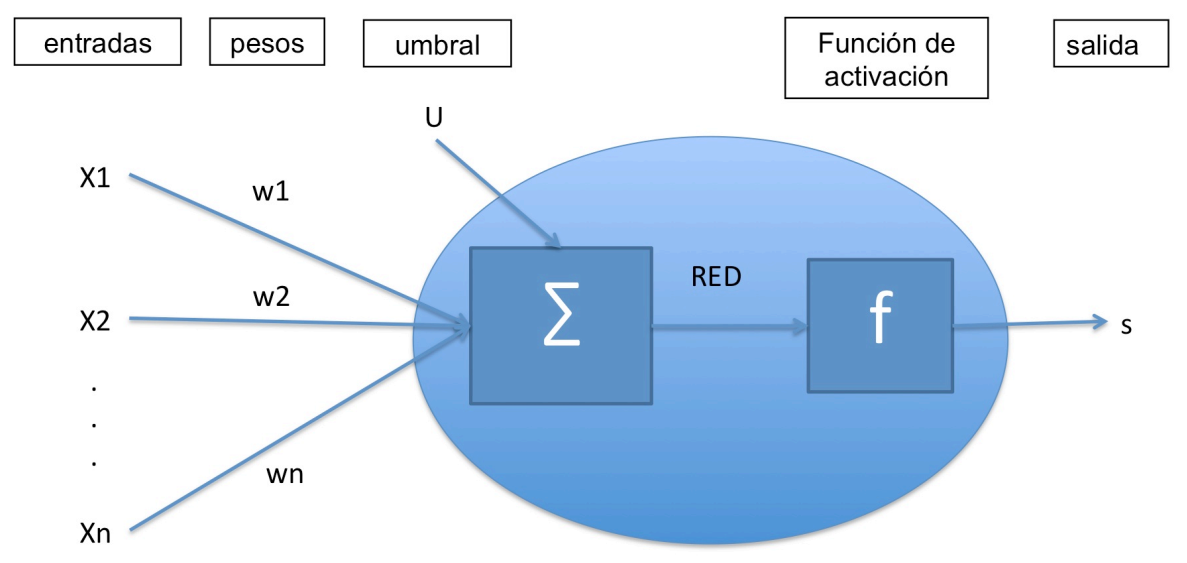
\includegraphics[scale=.2]{image-20210312101135112.png}}
\end{figure}
Las \textbf{entradas son los valores de los atributos}
(\(x_1,x_2,..,x_n\)) y un umbral, se hace \textbf{combinación lineal de
las entradas con unos pesos} (\(w_0+w_ix_1+...+w_nx_n\)) y se pasa el
\textbf{resultado por una función de activación} que nos da la salida.

\textbf{Tipos de función de activación:}

\begin{itemize}

\item
  Umbral, devuelve 0 o 1.
  \begin{figure}[H]
	\ffigbox[\FBwidth]
	{\caption{Función Umbral}}
	{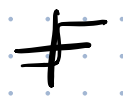
\includegraphics[scale=.8]{image-20210312101914163.png}}
\end{figure}
\item
  Lineal.
  \begin{figure}[H]
	\ffigbox[\FBwidth]
	{\caption{Función Lineal}}
	{\begin{tikzpicture}[scale=.5]
		\begin{axis}[
			title={Titulo},
			xlabel={Eje x},
			ylabel={Eje y},
			legend pos=north west,
			ymajorgrids=true,
			xmajorgrids=true,
			grid style=dashed,
		]
		\addplot[color=blue, mark=*]
			{x};
			\legend{Función}
			
		\end{axis}
	\end{tikzpicture}}
\end{figure}
\item
  Sigmoidal.
  \begin{figure}[H]
	\ffigbox[\FBwidth]
	{\caption{Función Sigmoidal}}
	{\begin{tikzpicture}[scale=.5]
		\begin{axis}[
			title={Titulo},
			xlabel={Eje x},
			ylabel={Eje y},
			legend pos=north west,
			ymajorgrids=true,
			xmajorgrids=true,
			grid style=dashed,
		]
		\addplot[color=blue, mark=*]
			{1/(1+exp(-x))};
			\legend{Función}
			
		\end{axis}
	\end{tikzpicture}}
\end{figure}
  
\item
  RELU, se ha visto que el aprendizaje es más rápido.
  \begin{figure}[H]
	\ffigbox[\FBwidth]
	{\caption{Función RELU}}
	{\begin{tikzpicture}[scale=.5]
		\begin{axis}[
			title={Titulo},
			xlabel={Eje x},
			ylabel={Eje y},
			legend pos=north west,
			ymajorgrids=true,
			xmajorgrids=true,
			grid style=dashed,
		]
		\addplot[color=blue, mark=*]
			{(x>=0)*x};
			\legend{Función}
			
		\end{axis}
	\end{tikzpicture}}
\end{figure}
\end{itemize}

El aprendizaje consiste en determinar los pesos que se aplican a las
entradas.

La regla que se aplica de forma habitual es la \textbf{Regla delta}, que
es parecido al descenso del gradiente. Se empieza con peso aleatorio y
con las iteraciones del entrenamiento se van actualizando los pesos.
\(w_i \leftarrow w_i+\Delta w_i\) El delta es una pequeña variación es
ŋ\((t-o)x_1\) donde ŋ es una tasa de aprendizaje, \(t\) la salida real y
\(o\) el valor que damos.

En general para hacer descenso del gradiente necesitamos que la función
sea derivable y con un único mínimo.

Se van metiendo los datos de entrada, se recibe la salida y según el
error se van actualizando los pesos, para cuando los pesos se
estabilizan.

\subsection{Perceptrón}

Es una forma más simple de red de neuronas, formada por una sola
neurona. Usa la función escalón como función de activación.

Se usa en tareas de clasificación lineal, es capaz de determinar el
hiperplano capaz de discriminar los ejemplos en dos clases.

\subsection{Redes}

Red neuronal multicapa
\begin{figure}[H]
	\ffigbox[\FBwidth]
	{\caption{Diagrama Red neuronal multicapa}}
	{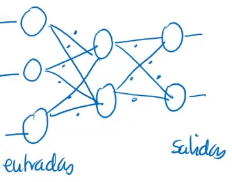
\includegraphics[scale=.85]{image-20210312102144206.png}}
\end{figure}

Es un \textbf{conjunto de neurona conectadas entre sí} que se
distribuyen en capas.

\textbf{Ventajas}:

\begin{itemize}

\item
  Son robustas ante el ruido.
\item
  Trabajan con datos complejos (difíciles de clasificar, como sensores)
\item
  Éxito en reconocimiento del habla y visión. Deep learning
\item
  Dan buenos resultados.
\end{itemize}

\textbf{Desventaja}: El aprendizaje es lento.

En las redes multicapa el cálculo del error se complica, hay varias
salidas y capas ocultas.

\subsection{Backpropagation o
Retropropagación}

Se basa en:
$Error \sim \sum _{d \in D} \sum_{k \in outputs} (t_{kd}-o_{kd})^2$.
Para cada ejemplo:

\begin{enumerate}
\def\labelenumi{\arabic{enumi}.}

\item
  Se propaga desde la \textbf{entrada hasta la salida} (calcular la
  salida de la red)
\item
  \textbf{Propagación del error hacia atrás}: En las que están en la
  última capa es fácil, pero para las que están en las capas intermedias
  no tanto.

  \begin{enumerate}
  \def\labelenumii{\arabic{enumii}.}
  
  \item
    Se calcula el \textbf{error en la unidad de salida}:
    \(\delta_k \leftarrow\) \(o_k(1-o_k)(t_k-o_k)\) Este valor es el
    (t-o) de la variación delta, en este caso para una función sigmoidal
    en vez de lineal
  \item
    \textbf{En las capas ocultas}: Se calcula con las unidades que están
    conectadas posteriormente,
    \(\delta_n \leftarrow o_n(1-o_n)\sum_{k \in output} w_{kn}\delta_k\)
  \end{enumerate}
\end{enumerate}

\subsection{Deep Learning}

Redes neuronales convolucionales. Se usan para procesado de imágenes.

\textbf{Puede recibir datos en crudo, no necesita que se los pasemos
como atributo valor}, lo que es una ventaja no hay que elegir los atributos
relevantes y organizar los datos. Recibe el grueso de los datos y los
va cogiendo por partes y agrupando, Convolution. Después se reduce la
resolución de la imagen, Pooling. Se repite el proceso hasta que tenemos
lo datos para clasificar, extracción de características, y podemos
generar una red neuronal totalmente conectada, classification.

\begin{figure}[H]
	\ffigbox[\FBwidth]
	{\caption{Diagrama de Deep Learning}}
	{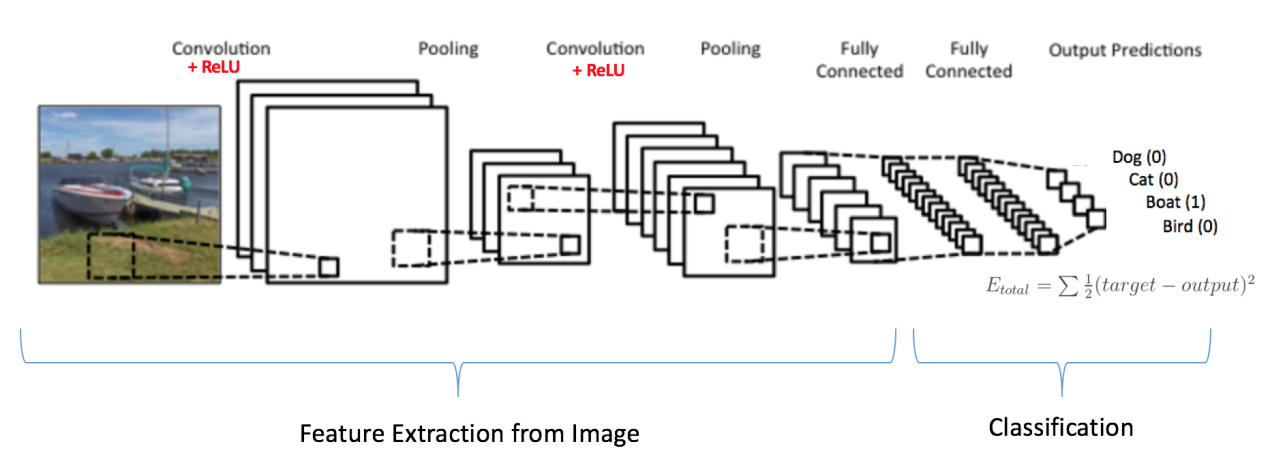
\includegraphics[scale=.3]{image-20210312111406573.png}}
\end{figure}

\section{Algoritmos genéticos}
\begin{figure}[H]
	\ffigbox[\FBwidth]
	{\caption{Diagrama Genético}}
	{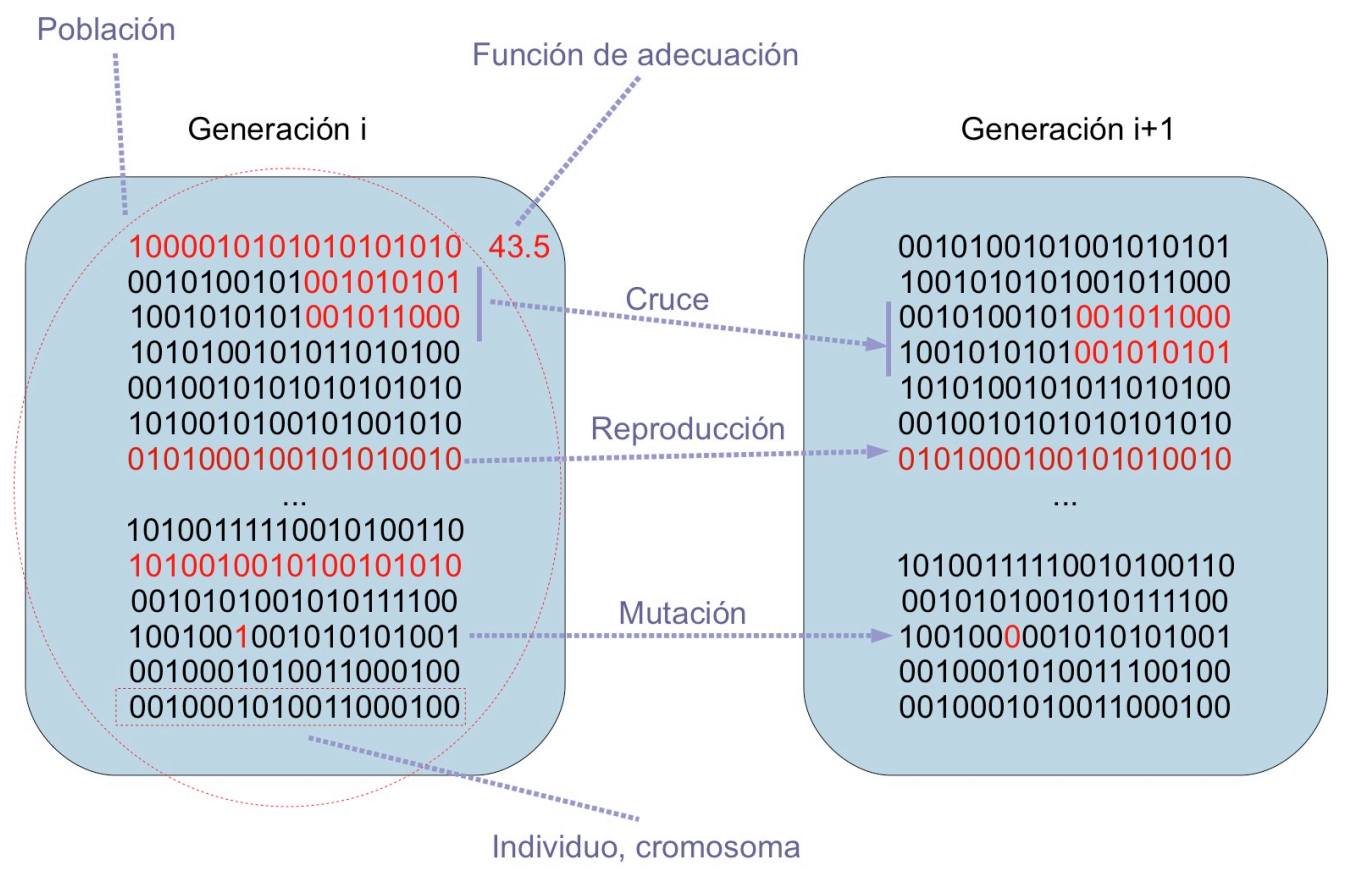
\includegraphics[scale=.4]{2021-03-19 11_26_59-otras-tecnicas.pdf - Foxit Reader.png}}
\end{figure}
Aprendizaje basado en evolución simulada, se mantiene una colección de soluciones, se evoluciona a través de generaciones por recombinación de las más adecuadas y eliminación de las menos adecuadas, y se termina cuando se obtiene una solución suficientemente adecuada.

\textbf{Son algoritmos de búsqueda local estocástica}, que las acciones tienen una probabilidad de ocurrir, son buenos para la optimización.

Hacen \textbf{búsqueda en el espacio de soluciones}, se usan cuando es fácil encontrar una solución, pero no la óptima. Funcionan por generaciones, en la que cada \textbf{generación} tiene una \textbf{población}, que está compuesta por p \textbf{individuos}, cada uno es una solución al problema.

\textbf{Factores clave:}
\begin{itemize}
  \item Elegir como representar los datos, se pueden utilizar cadenas de bits (llamado Genético) o alguna estructura de datos más compleja.
  \item Las operaciones para combinar soluciones y generar soluciones nuevas.
  \item La \textbf{función de adecuación (fitness)} que indica como de buena es una población, cuanto más es mejor. Transforma el genotipo (cadena de bits) en el fenotipo (significado de la cadena bits).
\end{itemize}

\textbf{Proceso:}
\begin{figure}[H]
	\ffigbox[\FBwidth]
	{\caption{Algoritmo genético}}
	{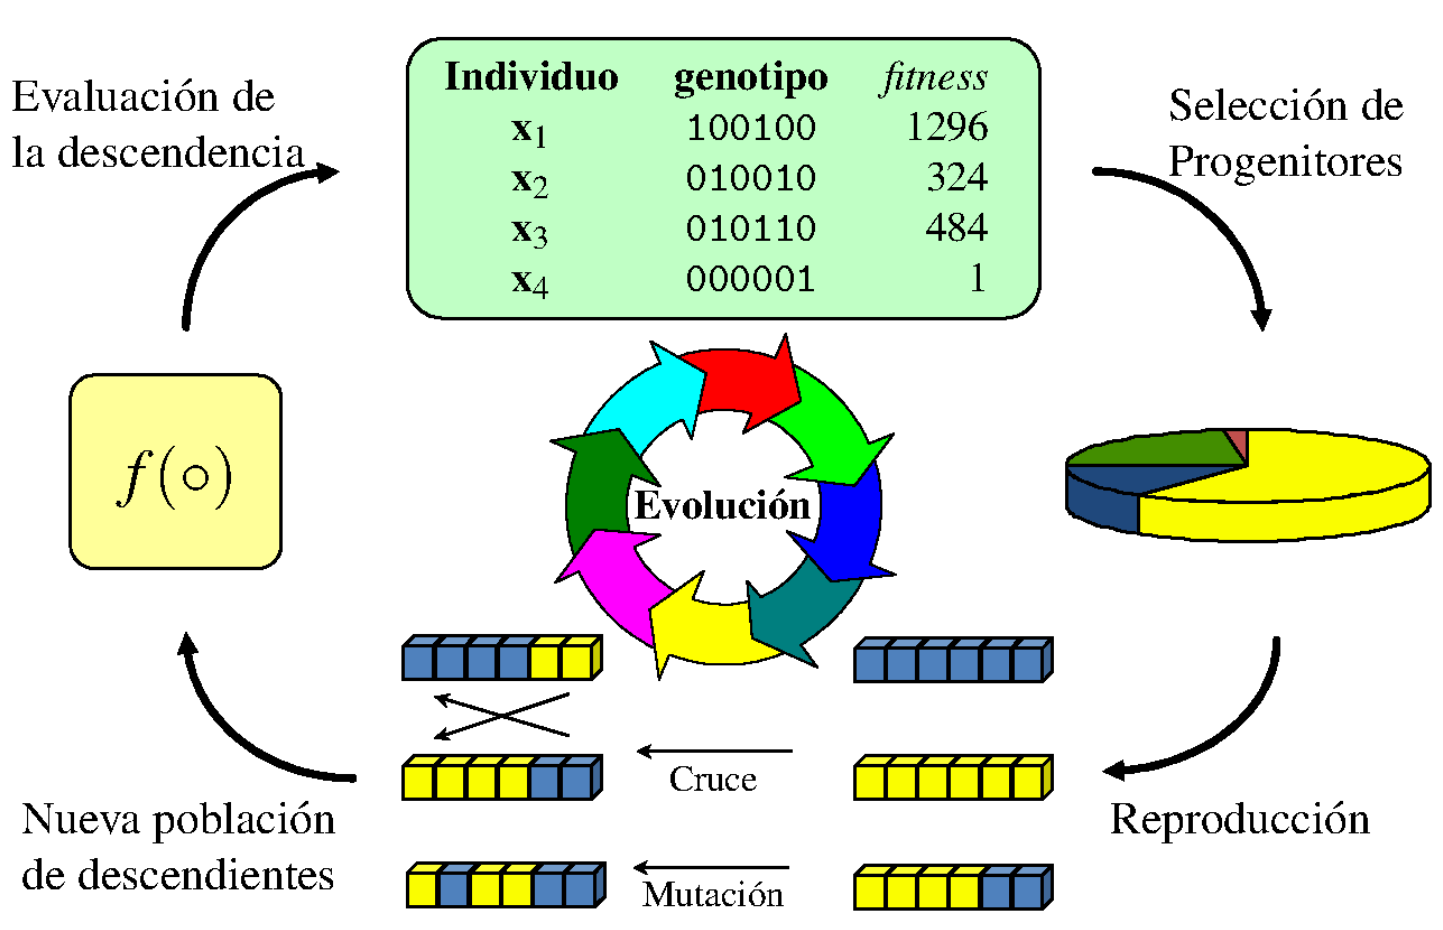
\includegraphics[scale=.3]{2021-03-19 11_42_34-otras-tecnicas.pdf - Foxit Reader.png}}
\end{figure}
\begin{enumerate}
  \item Se selecciona un conjunto de individuos de la población de soluciones. Se pueden elegir por Ruleta (por número aleatorio) o por Torneo (se coge un par de individuos y se escoge el mejor, dejando al otro fuera).
  \item A la nueva población se le realizan una serie de modificaciones como: reproducción, cruce, mutaciones y clone. Y quedan unos sobrevivientes, siempre tiene el mismo número de individuos.
  Cada operación tiene una probabilidad, por eso es búsqueda estocástica.
  \begin{description}
    \item[Cruze] Una parte de un par de individuos, mezcla de los progenitores.
    \item[Reproducción] Pasa a la nueva generación/población igual.
    \item[Mutación] Cambios muy pequeños, un solo bit.
  \end{description}
  \item Se evalúa la nueva población. Si es mejor pasa a ser la población base (generación), Si no se descarta y se intentan otras alternativas.
\end{enumerate}

\chapter{TEMA 5. Técnicas Vagas y No Supervisadas}
\section{Aprendizaje basado en instancias (IBL)}
No genera modelo, lo que hace es que cuando recibe un dato nuevo busca algunos similares de los conocidos.
\begin{figure}[H]
	\ffigbox[\FBwidth]
	{\caption{Estrategia IBL}}
	{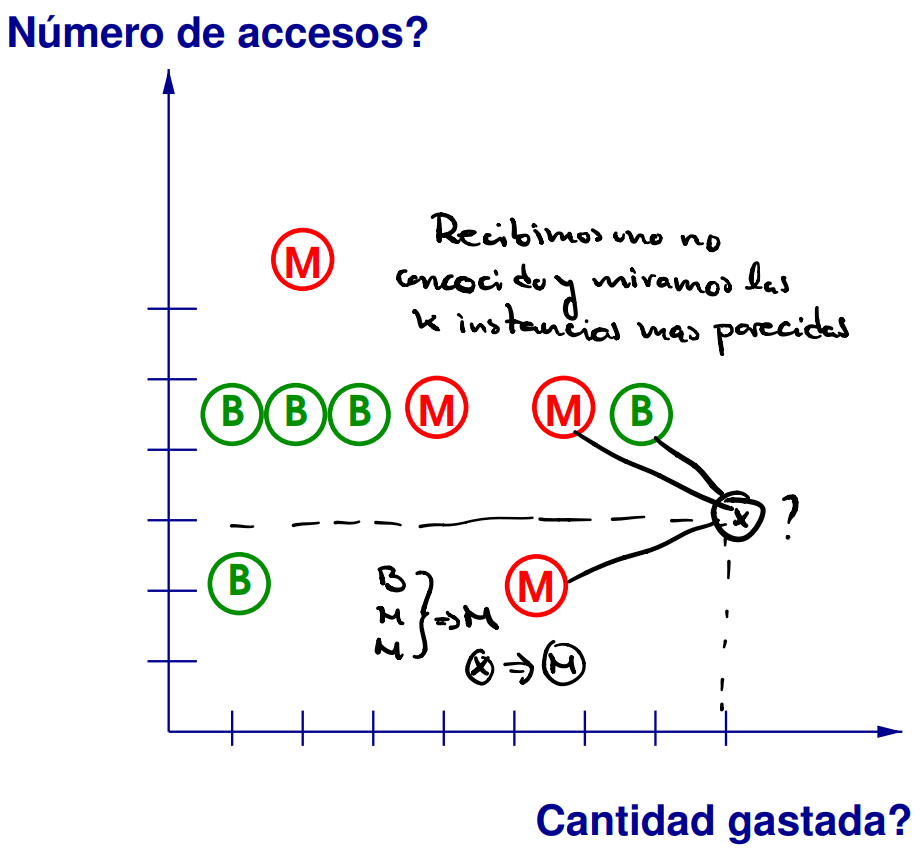
\includegraphics[scale=.3]{2021-03-19 12_05_34-Aprendizaje basado en instancias y no supervisados.pdf - Foxit Reader.png}}
\end{figure}
\textbf{Fases:}
\begin{enumerate}
  \item \textbf{Entrenamiento:} Almacenamiento de todo el conjunto de datos disponibles.
  \item \textbf{Generalización:} Cuando recibe un nuevo dato, se cogen un conjunto de datos similares, que son utilizados para clasificar el nuevo dato. Todo el computo se realiza en tiempo de clasificación, Aprendizaje Perezoso.
\end{enumerate}
Para definir similitud, se utilizan medidas de distancia (más cercano, más similares).

El algoritmo recibe como entrada k, que indica el número de vecinos más cercanos que se van a considerar (K-NN, K-Nearest Neighbors). 

\subsection{K-Nearest Neighbors}
Las instancias corresponden a puntos en un espacio de dimensión n (n atributos) y los vecinos más cercanos se calculan con la distancia euclídea ($d\left( \vec{x},\vec{z}\right)   = \sqrt {\sum _{i=1}^{n}  \left( x_{i}-z_{i}\right)^2 }$).

Si los atributos tienen diferentes rangos, se normalizan, y si son valores simbólicos, se define el valor por posible valor.
\subsection{Función Objetivo}
Dada una instancia x y sus k vecinos, nos indica cual es la clase. Dependiendo del tipo de valores se usan distintos métodos:
\begin{description}
  \item[Caso discreto (clasificación)] Valor más común de entre los k vecinos más cercanos. 
  $$ \hat{f}(\vec{x}) = \arg\max _{c \in C} \sum^k_{i=1} \delta(c,f(\vec{z^i}))$$
  \item[Caso continuo (regresión)] Valor medio de entre los k vecinos. 
  $$ \hat{f}(\vec{x}) = \frac{\sum^k_{i=1} f(\vec{z^i})}{k}$$
\end{description}
También se puede ponderar la importancia de cada vecino en el valor de la función objetivo, en función de su distancia. Donde $w_i = \frac{1}{d(\vec{x},\vec{z^i})^2}$.
\begin{description}
  \item[Caso discreto (clasificación)] $ \hat{f}(\vec{x}) = \arg\max _{c \in C} \sum^k_{i=1} w_i \times \delta(c,f(\vec{z^i}))$
  \item[Caso continuo (regresión)] Media ponderada. $ \hat{f}(\vec{x}) = \frac{\sum^k_{i=1} w_i f(\vec{z^i})}{\sum^k_{i=1} w_i}$
\end{description}

\subsection{Selección de los K vecinos}
El parámetro k identifica cuantos vecinos se utilizan para la decisión, su valor es el que mejor resultados aporta, no hay una regla que siempre funcione. Las regiones que se forman con 1-NN se denominan regiones de Voronoi.

Medidas de distancia:
\begin{description}
  \item[Distancia de Hamming (atributos no numéricos)] $\left(x_{m}-z_{m}\right)=\left\{\begin{array}{ll}0 & \text { si } x_{m}=z_{m} \\ 1 & \text { si } x_{m} \neq z_{m}\end{array}\right.$
  \item[Manhattan] $d(\vec{x}, \vec{z})=\sum_{m=1}^{n}\left|x_{m}-z_{m}\right|$
  \item[Minkowski] $d(\vec{x}, \vec{z})=\left(\sum_{m=1}^{n}\left|x_{m}-z_{m}\right|^{k}\right)^{\frac{1}{k}}$
\end{description}
\subsection{Propiedades}
\begin{itemize}
  \item Las instancias son puntos de un espacio n dimensional, donde n es el número de atributos.

  \item No hay muchos atributos por instancias, 20 aprox.

  \item Hay muchos datos de entrenamiento.

\end{itemize}

\subsubsection{Ventajas}
\begin{itemize}
  \item Simple e intuitivo.

  \item Fácil de usar.

  \item Funciona bien cuando la función objetivo es muy compleja.

  \item El entrenamiento es muy rápido.

  \item Efectivo si hay muchos ejemplos. Consistente asintóticamente: Con infinitos ejemplos y un k suficientemente grande, es capaz de aproximarse al mejor clasificador (Bayes óptimo).

\end{itemize}
\subsubsection{Problemas y sus soluciones}
\begin{itemize}
  \item Muy \textbf{sensible a atributos irrelevantes}
  \begin{itemize}
    \item \textbf{Selección de atributos:} Determinar qué características son las interesantes, y eliminar las restantes. Se pueden utilizar técnicas wrapper, que busca en el espacio de atributos, métodos estadísticos, algoritmos genéticos, etc.
    \item \textbf{Ponderación de atributos:} Es menos radical que eliminar atributos y consiste en dar el peso que minimice el error a los distintos atributos a la hora de seleccionar vecinos por distancia.
  \end{itemize}
 
  \item \textbf{Coste de clasificación alto (tiempo)}, no tarda en entrenar, pero cuando clasifica compara todos los ejemplos
  \begin{itemize}
    \item \textbf{Indexación:} Organizar el conjunto de instancias
    \begin{itemize}
      \item \textbf{Árboles KD (k dimensional):} Particionar el espacio en regiones marcadas por las instancias que tenemos, en el que cada rama va reduciendo el espacio. Alterna entre dimensiones.
      
      \begin{figure}[H]
        \ffigbox[\FBwidth]
        {\caption{Ejemplo Árbol KD}}
        {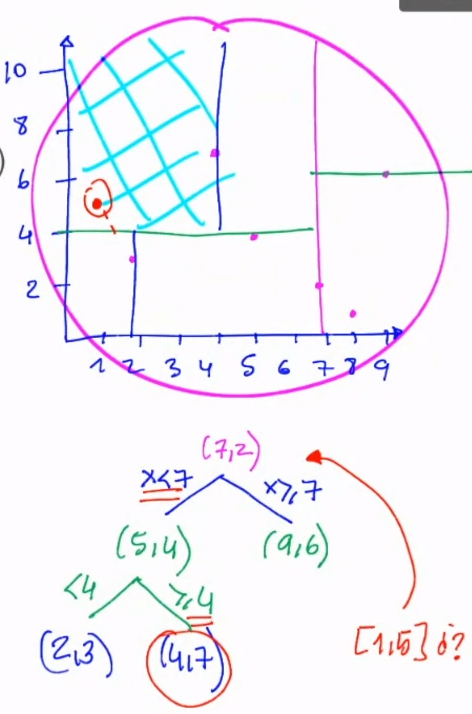
\includegraphics[scale=.7]{2021-03-19 14_58_39-AA IBL y no supervisados I.mkv.png}}
      \end{figure}

      \item \textbf{Agrupación o clustering:} Que es de aprendizaje no supervisado.
    \end{itemize}
  \end{itemize}
  \item \textbf{Almacenamiento (memoria) de todos los ejemplos}
  \begin{itemize}
    \item \textbf{Selección de instancias:} Elegir un grupo reducido de instancias (prototipos, ejemplos representativos) que mantengan la misma información que el conjunto total. Se puede hacer de manera incremental, desde el conjunto vacío e ir añadiendo, o decremental, desde el conjunto completo y eliminando. Se sigue un criterio para sacar o meter una instancia en el conjunto, que siga clasificando correctamente o se reduce las que clasifica mal.
    \item \textbf{Reemplazo de instancias:} Calcular prototipos a partir del conjunto de entrenamiento, y esos prototipos podrían sustituirse por los ejemplos que lo han generado. Se pueden generar con técnicas de clustering.
  \end{itemize}

\end{itemize}
\subsection{Otros métodos}
\subsubsection{Locally Weighted Regression}
En vez de devolver la media de la clase de los k vecinos, se crea un modelo lineal de forma local en zonas del espacio. Por cada consulta se obtienen los k vecinos y se crea el modelo de regresión lineal.

Se podría aplicar cualquier otro método de aproximación, como las redes neuronales.
\subsubsection{Case Based Reasoning}
Los ejemplos no son de la forma atributo-valor, sino que se representan con cualquier estructura de datos, como pueden ser imágenes, documentos, planos, etc. Consigue adaptar los datos de otros problemas al actual, viendo cómo se han resuelto problemas previos.


\section{Aprendizaje no supervisado}
No conocemos la clase, solo tenemos atributos en los ejemplos.

Lo que se hace es ver que instancias son parecidas y se crean grupos de instancias similares. También se utiliza para reducir el número de instancias y quedarnos con el más representativo del grupo.

\subsection{Posibles objetivos}
\begin{itemize}
  \item \textbf{Agrupación:} Dado un conjunto de ejemplos sin etiquetar, agruparlos según algún criterio.
  
  Ese criterio suele venir por:
  \begin{itemize}
    \item \textbf{Aprendizaje paramétrico:} Parámetros asumidos.
    \item \textbf{Aprendizaje no paramétrico:} Alguna medida de distancia.
  \end{itemize}
  POR COMPLETAR
  \item \textbf{Indexación:} Dado un conjunto de ejemplos, facilitar su acceso organizándolos.
  \item \textbf{Asociación:} Dados unos datos, establecer relaciones y/asociaciones entre datos.
  \item \textbf{Generación de jerarquías:} Dados unos datos en un mismo nivel, generar jerarquías en dichos datos.
  \item \textbf{Reducción de dimensionalidad:} Dados unos datos, reducir la dimensión o número de atributos que caracterizan los datos.
  \item \textbf{Visualización:} Dados unos datos con representación compleja, permitir su visualización.
\end{itemize}

\end{document}
